% ============================================================
%  thesis_main.tex
%  "Multi-Agent Proximal Policy Optimization for Adaptive
%   Traffic Signal Control: Stress-Testing on Real-World
%   Baku Intersection Scenarios"
%
%  ADA University — Master of Science Thesis
%  School of Information Technology and Engineering
%
%  Compile:
%    pdflatex thesis_main
%    bibtex   thesis_main
%    pdflatex thesis_main
%    pdflatex thesis_main
% ============================================================

\documentclass[12pt,oneside,a4paper]{report}

% ── Page geometry ────────────────────────────────────────────
\usepackage[a4paper,
            top    = 1.0in,
            bottom = 1.0in,
            left   = 1.5in,    % extra left margin for binding
            right  = 1.0in]{geometry}

% ── Typography ───────────────────────────────────────────────
\usepackage{mathptmx}          % Times New Roman body + math
\usepackage[T1]{fontenc}
\usepackage[utf8]{inputenc}
\usepackage{microtype}

% ── Line spacing ─────────────────────────────────────────────
\usepackage{setspace}
\onehalfspacing                % 1.5 line spacing for body

% ── Mathematics ──────────────────────────────────────────────
\usepackage{amsmath,amssymb,amsfonts}

% ── Graphics & colours ───────────────────────────────────────
\usepackage{graphicx}
\usepackage{xcolor}
\usepackage{float}

% ── Tables ───────────────────────────────────────────────────
\usepackage{booktabs}
\usepackage{multirow}
\usepackage{array}
\usepackage{tabularx}

% ── Captions ─────────────────────────────────────────────────
\usepackage[font=small, labelfont=bf,
            justification=centering]{caption}

% ── PGFPlots / TikZ ──────────────────────────────────────────
\usepackage{pgfplots}
\usepackage{pgfplotstable}
\usepackage{tikz}
\pgfplotsset{compat=1.18}
\usetikzlibrary{shapes.geometric,arrows.meta,positioning,
                fit,backgrounds}

% ── Headers / footers ────────────────────────────────────────
\usepackage{fancyhdr}
\pagestyle{fancy}
\fancyhf{}
\fancyfoot[C]{\thepage}
\renewcommand{\headrulewidth}{0pt}
\setlength{\headheight}{14pt}
\fancypagestyle{frontmatter}{%
  \fancyhf{}
  \fancyfoot[C]{\thepage}
  \renewcommand{\headrulewidth}{0pt}
}

% ── TOC customisation ─────────────────────────────────────────
\usepackage{tocloft}
\renewcommand{\contentsname}{Table of Contents}
\renewcommand{\cftchapfont}{\bfseries}
\renewcommand{\cftchappagefont}{\bfseries}
\setlength{\cftbeforechapskip}{6pt}

% ── Chapter heading style ────────────────────────────────────
\usepackage{titlesec}
\titleformat{\chapter}[hang]
  {\normalfont\Huge\bfseries}
  {\thechapter.}{0.6em}{}
\titlespacing*{\chapter}{0pt}{0pt}{18pt}

% ── URLs & links ─────────────────────────────────────────────
\usepackage{url}
\usepackage[colorlinks=true,
            linkcolor=black,
            citecolor=black,
            urlcolor=blue]{hyperref}
\usepackage{doi}

% ── Miscellaneous ────────────────────────────────────────────
\usepackage{enumitem}
\usepackage{parskip}
\setlength{\parindent}{0.5in}
\setlength{\parskip}{0pt}

% ── Macros ───────────────────────────────────────────────────
\newcommand{\ppo}{\textsc{PPO}}
\newcommand{\ft}{\textsc{FT}}
\newcommand{\sumo}{\textsc{SUMO}}
\newcommand{\marl}{\textsc{MARL}}
\newcommand{\atsc}{\textsc{ATSC}}
\newcommand{\rl}{\textsc{RL}}

% ============================================================

% Enable DOI/URL output in IEEEtran bibliography
\begin{filecontents*}{IEEEtranBSTCTL.bib}
@IEEEtranBSTCTL{BSTcontrol,
  CTLuse_forced_etal       = {no},
  CTLmax_names_forced_etal = {10},
  CTLnames_show_etal       = {10},
  CTLuse_url               = {yes},
  CTLuse_doi               = {yes}
}
\end{filecontents*}

\begin{document}
\sloppy
% ── Front matter (Roman numerals) ────────────────────────────
\pagenumbering{roman}
\pagestyle{fancy}

% ============================================================
% COVER PAGE
% ============================================================
\begin{titlepage}
  \begin{center}
    \vspace*{0.2in}
    {\Large\bfseries ADA UNIVERSITY}\\[6pt]
    {\large SCHOOL OF INFORMATION TECHNOLOGY AND ENGINEERING}\\[2pt]
    {\normalsize Master of Science in Computer Science}

    \vspace{0.6in}
    \rule{\textwidth}{1.5pt}\\[8pt]
    {\LARGE\bfseries
      Multi-Agent Proximal Policy Optimization\\[4pt]
      for Adaptive Traffic Signal Control:\\[4pt]
      Stress-Testing on Real-World\\[4pt]
      Baku Intersection Scenarios}\\[8pt]
    \rule{\textwidth}{1.5pt}

    \vspace{0.6in}
    {\normalsize
      A Thesis Submitted in Partial Fulfillment of the\\
      Requirements for the Degree of\\[6pt]
      \textbf{Master of Science in Computer Science}}

    \vspace{0.6in}
    {\normalsize by}\\[8pt]
    {\Large\bfseries Abdullah Kazimov}\\[4pt]
    {\normalsize \texttt{akazimov14095@ada.edu.az}}

    \vspace{0.6in}
    \begin{tabular}{rl}
      \textbf{Supervisor:} & Dr.\ Jamaladdin Hasanov \\
                           & Assistant Professor      \\
                           & School of IT and Engineering \\
                           & ADA University           \\
    \end{tabular}

    \vfill
    {\normalsize Baku, Azerbaijan \hfill April 2026}
  \end{center}
\thispagestyle{fancy}
\end{titlepage}
\setcounter{page}{2}

% ============================================================
% APPROVAL PAGE
% ============================================================
\clearpage
\thispagestyle{fancy}
\begin{center}
  {\Large\bfseries ADA UNIVERSITY}\\[4pt]
  {\large SCHOOL OF INFORMATION TECHNOLOGY AND ENGINEERING}

  \vspace{0.4in}
  {\large\bfseries THESIS APPROVAL FORM}

  \vspace{0.3in}
  \begin{tabular}{@{}lp{3.8in}@{}}
    \textbf{Thesis Title:} &
      Multi-Agent Proximal Policy Optimization for Adaptive Traffic
      Signal Control: Stress-Testing on Real-World Baku
      Intersection Scenarios \\[10pt]
    \textbf{Student Name:} & Abdullah Kazimov \\[10pt]
    \textbf{Student ID:}   & 14095 \\[10pt]
    \textbf{Program:}      & Master of Science in Computer Science \\[10pt]
    \textbf{Submission Date:} & April 2026 \\
  \end{tabular}
\end{center}

% ============================================================
% ABSTRACT (3rd page)
% ============================================================
\clearpage
\thispagestyle{fancy}
\begin{center}
  {\Large\bfseries ABSTRACT}
\end{center}

\noindent
Urban traffic congestion remains a persistent challenge in fast-growing
cities, where fixed-time signal plans cannot adjust to the randomness
and variability of real traffic demand. This thesis investigates whether
a multi-agent reinforcement learning (\marl{}) approach can improve
adaptive traffic signal control (\atsc{}) on realistic road networks
rather than on simplified synthetic benchmarks. To answer that question,
it trains and evaluates a Proximal Policy Optimization (\ppo{})-based
control framework on four real-topology traffic scenarios derived from
Baku street networks and simulated in the open-source \sumo{} platform.

The four scenarios were designed to reflect substantially different
operating conditions: a high-load bottleneck corridor, a three-intersection
arterial, a mixed-mode pedestrian junction, and a twelve-light hexagonal
highway sub-network. For each scenario, the observation and action spaces
were trimmed to the active topology, and the policy was trained for
approximately 500{,}000 environment decision steps using Stable-Baselines3.
Performance was then evaluated against a fixed-time \sumo{} baseline using
a multi-seed protocol with five to ten independent demand seeds per
scenario. The comparison focuses on four metrics: stopped-vehicle ratio,
average waiting time, average queue length, and throughput.

The results show that \ppo{} delivers consistent improvements across all
four scenarios. Mean throughput gains range from $+16.7\%$ to $+31.1\%$,
stopped-vehicle ratio improves by $+8.6\%$ to $+19.4\%$, and waiting time
improves by as much as $+24.8\%$ in the Bottleneck scenario. The analysis
also reveals a near-perfect Pearson correlation ($r = 0.9948$) between
stopped-vehicle ratio and queue length, suggesting that these measures
capture closely related aspects of congestion. In addition, the experiments
show that a carefully balanced seven-term reward function is essential for
stable learning across all four scenarios.

Overall, the study demonstrates that deep reinforcement learning can
outperform classical fixed-time control on realistic, city-derived traffic
networks when the reward design is well calibrated and the state-action
representation is matched to the underlying topology.

\vspace{0.3in}
\noindent\textbf{Keywords:}
adaptive traffic signal control, multi-agent reinforcement
learning, proximal policy optimization, SUMO simulation,
reward shaping, urban congestion, Baku road network,
stress testing, multi-seed evaluation

% ============================================================
% ACKNOWLEDGEMENTS
% ============================================================
\chapter*{Acknowledgements}
\addcontentsline{toc}{chapter}{Acknowledgements}

I would like to express my sincere gratitude to my supervisor,
Dr.\ Jamaladdin Hasanov, for his guidance, encouragement, and
thoughtful feedback throughout this research.

I am also deeply grateful to the Center for Data Analytics and
Research Lab for providing the computational resources that made
the experiments in this thesis possible.

My thanks also go to the \sumo{} development team for maintaining an
excellent open-source microsimulation platform, and to the
Stable-Baselines3 community for providing reliable and reproducible
deep reinforcement learning implementations that greatly reduced the
engineering overhead of this work.

Finally, I gratefully acknowledge the open-source community whose
tools and libraries --- including PyTorch, Gymnasium, NumPy, and
Matplotlib --- formed the technical foundation of this study.


% ============================================================
% TABLE OF CONTENTS
% ============================================================
\clearpage
\pagestyle{fancy}
\tableofcontents

\clearpage
\listoffigures
\addcontentsline{toc}{chapter}{List of Figures}

\clearpage
\listoftables
\addcontentsline{toc}{chapter}{List of Tables}

% ── Abbreviations ────────────────────────────────────────────
\clearpage
\chapter*{List of Abbreviations}
\addcontentsline{toc}{chapter}{List of Abbreviations}
\begin{singlespace}
\begin{tabbing}
  \hspace{2.2in}\= \kill
  \textbf{ATSC}  \> Adaptive Traffic Signal Control \\
  \textbf{DQN}   \> Deep Q-Network \\
  \textbf{DDPG}  \> Deep Deterministic Policy Gradient \\
  \textbf{DRL}   \> Deep Reinforcement Learning \\
  \textbf{GAE}   \> Generalized Advantage Estimation \\
  \textbf{GNN}   \> Graph Neural Network \\
  \textbf{LSTM}  \> Long Short-Term Memory \\
  \textbf{MARL}  \> Multi-Agent Reinforcement Learning \\
  \textbf{MDP}   \> Markov Decision Process \\
  \textbf{MLP}   \> Multi-Layer Perceptron \\
  \textbf{PPO}   \> Proximal Policy Optimization \\
  \textbf{RL}    \> Reinforcement Learning \\
  \textbf{SB3}   \> Stable-Baselines3 \\
  \textbf{SUMO}  \> Simulation of Urban MObility \\
  \textbf{TL}    \> Traffic Light \\
  \textbf{TraCI} \> Traffic Control Interface \\
  \textbf{FT}    \> Fixed-Time (control baseline) \\
\end{tabbing}
\end{singlespace}

% ============================================================
% BODY — continue Roman numerals throughout
% ============================================================
\clearpage

% ============================================================
\chapter{Introduction}
\label{chap:intro}
% ============================================================

\section{Definition of the Problem}
\label{sec:def}

Traffic signal control at urban intersections is one of the oldest
and most consequential problems in transportation engineering.  Since
the introduction of electronically controlled traffic lights in the
1920s, the dominant paradigm has remained largely unchanged: a
\emph{fixed-time} control plan assigns predetermined durations to each
green phase based on historical average traffic volumes, repeating the
same cycle regardless of the actual demand at any given moment.  While
this approach is simple, deterministic, and easy to maintain, it is
fundamentally incapable of responding to the stochastic, non-stationary
nature of real traffic flows.

In a fixed-time system, signal cycles are computed offline using
models such as Webster's optimal cycle formula~\cite{lammerhelbing2008},
which minimises average delay under the assumption of steady-state
Poisson arrivals.  This assumption breaks down in practice in at least
three important ways.  First, traffic demand exhibits strong temporal
variation --- morning and evening peak hours bring flows that are three
to five times higher than off-peak levels, and no single cycle length
is optimal for all conditions simultaneously.  Second, incident-driven
demand spikes (road works, accidents, public events) produce transient
congestion that a pre-programmed plan cannot mitigate.  Third,
multi-intersection corridors suffer from \emph{green-wave cascade
failures}: when one intersection becomes saturated, queues spill back
upstream and disrupt the carefully timed offsets of downstream signals,
causing system-wide delay that is disproportionately large relative to
the initial overload.

Baku, the capital of Azerbaijan, exemplifies these challenges with
particular urgency.  With a metropolitan population exceeding four
million and a registered vehicle fleet that has grown by more than
$60\%$ over the past decade, the city's arterial network is routinely
saturated during peak hours.  Key corridors such as H.\,Aliyev Avenue,
Neftchilar Avenue, and the ring roads surrounding the Old City
experience stop-and-go conditions for several hours daily.  The
fixed-time signal plans currently operating at most Baku intersections
were designed for traffic volumes that are substantially lower than
current demand, and their manual re-calibration is both expensive
and infrequent.

The problem addressed in this thesis can therefore be stated
precisely as follows:

\begin{quote}
\textit{Given a multi-intersection urban road network with stochastic,
time-varying vehicle demand, can a reinforcement learning agent, trained
entirely within a simulation environment, learn a signal timing policy
that consistently outperforms a fixed-time baseline across a diverse
set of demand seeds and intersection topologies?}
\end{quote}

Answering this question requires not only training a capable RL agent,
but also evaluating it honestly --- across multiple random seeds,
in four structurally different intersection scenarios, and on four
complementary performance metrics --- so that the result is
statistically credible rather than an artefact of a single
favourable evaluation condition.

\section{Objective of the Study}
\label{sec:obj}

The main goal of this study is to design, implement, and carefully
evaluate a multi-agent Proximal Policy Optimization framework for
adaptive traffic signal control using four real-topology Baku
intersection scenarios. To support that overall goal, the study
pursues the following specific objectives:

\begin{enumerate}[leftmargin=*, label=\textbf{O\arabic*.}]

  \item \textbf{Scenario development.}
        Construct four SUMO simulation scenarios whose road
        topologies are faithful to real Baku city segments, covering
        a complexity range from two traffic lights to twelve, and
        encompassing three distinct flow regimes: arterial corridors,
        pedestrian-mixed junctions, and highway sub-networks.

  \item \textbf{Environment engineering.}
        Design a Gymnasium-compatible simulation wrapper
        (\texttt{BakuSUMOEnv}) that exposes a trimmed, scenario-specific
        observation and action space, eliminating gradient noise from
        unused policy heads and making the learning problem tractable
        for a standard MLP policy.

  \item \textbf{Reward function design.}
        Derive a composite, multi-objective reward function using
        statistical gradient analysis, incorporating terms for
        throughput, congestion, hotspot detection, coordination
        balance, and phase fairness, anchored to an empirical B2
        baseline computed from fixed-time passive rollouts.

  \item \textbf{Policy training.}
        Train a shared \ppo{} agent on each scenario for approximately
        500{,}000 cumulative environment decision steps using
        Stable-Baselines3 with VecNormalize and SubprocVecEnv
        parallelism.

  \item \textbf{Multi-seed evaluation.}
        Evaluate the trained policy against the fixed-time baseline
        using a matched-snapshot protocol on five to ten independent
        demand seeds per scenario, reporting improvements on all four
        traffic metrics.

  \item \textbf{Analysis.}
        Quantify metric correlations, perform ablation studies on
        the action space and reward design, and analyse time-of-day
        performance patterns to explain \emph{when} and \emph{why}
        the RL agent outperforms fixed-time control.

\end{enumerate}

\section{Significance of the Problem}
\label{sec:sig}

The significance of this research operates at three levels:
practical, scientific, and local.

\subsection*{Practical Significance}

Traffic congestion imposes enormous economic costs.  A study by
INRIX estimates that American commuters lost an average of 99 hours
to traffic in 2022, at an aggregate cost of \$87 billion in lost
productivity~\cite{haydari2022survey}.  In rapidly urbanising
developing cities, these costs are proportionally even higher because
infrastructure investment lags population growth.  Signal timing
optimisation has been identified by the US Federal Highway
Administration as one of the most cost-effective traffic management
interventions, with benefit-to-cost ratios of up to $40:1$ for
adaptive systems versus fixed-time plans.

Beyond economic costs, traffic congestion generates significant
environmental externalities.  Stop-and-go driving at saturated
intersections increases fuel consumption by $15$--$30\%$ relative
to free-flow conditions, and urban signalised intersections are
responsible for a disproportionate share of localised particulate
matter and $\mathrm{NO}_x$ emissions~\cite{haydari2022survey}.
An adaptive signal controller that reduces average waiting time
therefore simultaneously reduces both congestion and emissions.

\subsection*{Scientific Significance}

The scientific contribution of this work addresses two persistent
gaps in the deep reinforcement learning for traffic signal control
(DRL-ATSC) literature.  First, the overwhelming majority of
published DRL-ATSC results are evaluated on idealised, symmetric
single-intersection grids~\cite{intellilight2018, presslight2019,
mplight2020}.  These synthetic environments maximise re-deployability
of benchmarks but systematically underestimate the difficulty of
real urban networks, where asymmetric lane counts, mixed
vehicle-pedestrian phases, and multi-intersection coordination are
the norm.  This thesis contributes a \emph{stress-tested} evaluation
on four structurally diverse, city-derived scenarios --- a
substantially harder benchmark.

Second, this work introduces and validates a \emph{multi-seed
evaluation protocol} as a necessary standard for honest assessment
of DRL-ATSC policies.  Because traffic demand is stochastic, a
single evaluation seed can produce a misleadingly positive or
negative result.  The multi-seed protocol developed here, covering
five to ten independent demand realisations per scenario, provides
a statistically credible picture of policy robustness.

\subsection*{Local Significance}

For Azerbaijan specifically, this thesis represents one of the first
academic studies applying deep reinforcement learning to signalised
intersections based on real Baku road topology.  The SUMO scenarios
developed are directly importable from the city's OpenStreetMap~\cite{openstreetmap2008}
export, meaning the trained policies could, in principle, be
transferred to real-world signal hardware with sensor integration
and safety validation work --- a deployment pathway described in
detail in Chapter~\ref{chap:results}.

\section{Review of Significant Research}
\label{sec:review_intro}

The application of machine learning to traffic signal control has
a history spanning more than three decades.  Abdulhai
et~al.~\cite{abdulhai2003} pioneered the use of Q-learning at a
single isolated intersection, reporting improvements of up to $34\%$
in average delay over a fixed-time baseline.  This seminal result
established the feasibility of RL for ATSC but left open the
question of scalability to multi-intersection networks.

The advent of deep learning as a function approximator unlocked a
new generation of DRL-ATSC methods.  IntelliLight~\cite{intellilight2018}
and PressLight~\cite{presslight2019} demonstrated that convolutional
and fully-connected deep Q-networks could outperform both fixed-time
and max-pressure baselines on city-scale datasets.  MPLight~\cite{mplight2020}
extended this paradigm to thousands of intersections via parameter
sharing, achieving near-linear scalability.  These works, however,
shared a common limitation: their evaluation environments were
large synthetic grids with uniform intersection geometries, making
their results difficult to interpret for real-world deployments
where heterogeneous topologies are the rule.

On the multi-agent coordination side, Chu~et~al.~\cite{chu2020marl}
showed that independent A2C agents with shared parameters can scale
to hundreds of intersections without explicit communication, while
MADDPG~\cite{maddpg2017} and QMIX~\cite{qmix2018} explored
centralised training with decentralised execution for better
credit assignment in cooperative settings.  A comprehensive
survey by Haydari and Y{\i}lmaz~\cite{haydari2022survey} identified
reward shaping, safe exploration, and real-world transferability
as the three most critical open problems in the field --- precisely
the challenges that motivate the design choices in this thesis.

A detailed critical review of all significant related work,
organised by research thread, is presented in Chapter~\ref{chap:lit}.

\section{Assumptions and Limitations}
\label{sec:assumptions}

The following assumptions underpin the experimental design and
must be kept in mind when interpreting the results.

\subsection*{Simulation Fidelity}

All experiments are conducted within SUMO, a microscopic traffic
simulator.  While SUMO models individual vehicle dynamics,
lane-changing, and gap-acceptance behaviour with high fidelity,
it remains a simulation.  Real traffic exhibits phenomena ---
such as aggressive gap-forcing, pedestrian jaywalking, and
sensor noise --- that are not fully captured.  The trained policy
has not been tested on hardware.

\subsection*{Semi-Synthetic Demand}

Vehicle demand is generated using time-of-day density functions
and turning ratios calibrated from Baku OpenStreetMap data,
not from recorded vehicle trajectories.  The absolute demand levels
are therefore approximate.  Relative comparisons between \ppo{} and
\ft{} under the same demand seed are unaffected by this assumption.

\subsection*{Training Seed Fixity}

Training uses seed 42 exclusively.  The policy is not ensemble-trained
across multiple initialisation seeds.  Some residual training variance
may therefore exist, though the multi-seed \emph{evaluation} protocol
mitigates this concern by testing the trained policy across ten
independent demand realisations for the primary benchmark.

\subsection*{Topology Specificity}

The trimmed observation and action spaces are scenario-specific.
A policy trained on the \textit{main} scenario (3 TLs) cannot be
directly transferred to the \textit{hexagon} scenario (12 TLs).
Each deployment target requires a dedicated training run.  This is
a deliberate design choice prioritising realism over redeployability,
as discussed in Section~\ref{sec:disc_limitations}.

\subsection*{Normalization Semantics}

Training rewards visible in SB3 logs are VecNormalize-scaled and
are not directly comparable to the raw SUMO metric improvements
reported in the results chapter.  All quantitative conclusions
are drawn from raw, unnormalized metrics collected with
\texttt{training=False, norm\_reward=False} at evaluation time.

% ============================================================
\chapter{Literature Review}
\label{chap:lit}
% ============================================================

\section{Classical Traffic Signal Control Methods}
\label{sec:lit_classical}

The foundation of modern traffic signal control was laid by
Webster~\cite{lammerhelbing2008}, who in 1958 derived an analytical
formula for the cycle length that minimises average vehicle delay
at an isolated, under-saturated intersection.  Webster's formula
remains the mathematical basis for most deployed fixed-time signal
plans worldwide.  Its key insight is that delay is a convex function
of the cycle length, with a unique minimum that depends on the
saturation flow and the demand-to-capacity ratio of each phase.
However, the formula assumes Poisson arrivals at a steady
rate --- an assumption that is violated during peak hours, in
oversaturated conditions, and whenever demand is non-stationary.

Adaptive extensions of the fixed-time paradigm were developed to
address this limitation.  SCOOT (Split Cycle Offset Optimisation
Technique) adjusts cycle lengths, splits, and offsets in real time
using detector data, operating as an outer loop around a
fixed-time plan.  SCATS (Sydney Coordinated Adaptive Traffic System)
similarly adjusts cycle parameters based on measured degree of
saturation.  While these systems represent a significant improvement
over static plans, they remain fundamentally reactive and rule-based:
their control laws are hand-engineered functions of measured
occupancy, and they do not generalise to demand patterns not seen
during calibration.

Max-pressure control~\cite{varaiya2013,presslight2019} provides a theoretical
throughput guarantee for under-saturated networks: by activating the
phase that maximises the pressure differential between incoming and
outgoing queues, the controller is provably stable in the sense that
queues remain bounded whenever demand is below capacity.  This
approach requires only queue length measurements at every lane and
no parameter tuning, making it attractive for deployment.  Its
limitation is that it optimises for throughput only, ignoring other
metrics such as average waiting time or pedestrian phase fairness,
and it does not learn from past experience --- it cannot anticipate
recurring demand patterns.

\section{Reinforcement Learning for Traffic Signal Control}
\label{sec:lit_rl_early}

The application of reinforcement learning to traffic signal control
was first explored in the 1990s.  Reinforcement learning frames
the signal timing problem as a Markov Decision Process (MDP)
in which the agent observes the state of the intersection
(typically queue lengths or occupancy ratios), selects a green
phase, and receives a reward signal derived from a congestion
metric~\cite{sutton_barto2018}.

Abdulhai et~al.~\cite{abdulhai2003} applied tabular Q-learning
~\cite{qlearning1992} to a single isolated intersection modelled in
a microscopic simulator, discretising the state space into bins
of queue length.  They reported reductions in average delay of
$26$--$34\%$ relative to fixed-time control, establishing the
proof of concept for RL-ATSC.  However, tabular Q-learning scales
exponentially in the number of state variables, limiting it to
single intersections with coarsely discretised observations.

Subsequent work explored alternative RL algorithms at the
single-intersection scale.  Fuzzy logic controllers were combined
with RL to handle the imprecision inherent in detector readings.
Actor-critic methods were proposed to reduce the high variance of
policy-gradient updates.  SARSA was applied alongside Q-learning
as an on-policy alternative.  Despite these advances, the
fundamental scalability barrier of tabular methods prevented
progress to multi-intersection coordination.

\section{Deep Reinforcement Learning for ATSC}
\label{sec:lit_deep}

The convergence of deep learning~\cite{deeplearning2015} and
reinforcement learning enabled a qualitative leap in ATSC
capabilities.  Deep Q-Networks (DQN)~\cite{dqn2015} replaced the
tabular Q-function with a deep neural network, enabling continuous
state spaces and high-dimensional observations.  The experience
replay buffer~\cite{per2016} and target network stabilisation techniques
introduced in DQN were critical for stable training on complex
environments.

\textbf{IntelliLight}~\cite{intellilight2018} introduced a
phase-based DQN formulation for traffic signal control that uses
lane-level queue and occupancy features as the state representation.
Its key innovation was the \emph{movement-based} action space,
which selects signal phases as combinations of compatible vehicle
movements rather than as arbitrary programme indices.  IntelliLight
reported improvements of up to $38\%$ in average travel time over
fixed-time baselines on synthetic New York City grid data.

\textbf{PressLight}~\cite{presslight2019} unified the theoretical
max-pressure objective with a deep RL reward signal, achieving
city-scale coordination on hundreds of intersections.  By tying the
RL reward to the max-pressure criterion, the authors demonstrated
that learned policies can inherit the stability guarantees of
max-pressure while also capturing fine-grained timing distinctions
that a purely rule-based approach misses.  Double DQN~\cite{doubledqn2016}
was adopted to reduce Q-value overestimation in the deep network.
Subsequent improvements---dueling network architectures~\cite{dueling2016},
noisy networks for exploration~\cite{noisynets2018}, and the Rainbow
combination of all these advances~\cite{rainbow2018}---further strengthened
the DQN family, though they are rarely adopted in ATSC due to the discrete
phase-selection action space.

\textbf{FRAP}~\cite{frap2019} introduced a phase-competition mechanism
in which signal phases compete pairwise based on their relative demand,
achieving both faster convergence and symmetry-invariant policies compared
to prior DQN formulations.

\textbf{MPLight}~\cite{mplight2020} extended the PressLight framework
to 2{,}510 intersections in Hangzhou and New York City via parameter
sharing: all agents share a single policy network that is conditioned
on the local intersection state.  This decentralised execution with
shared parameters approach was shown to scale near-linearly, with
coordination quality improving as more intersections are included
due to the reduced congestion externalities.

On the policy-gradient side, A3C~\cite{a3c2016} was applied to
traffic control with asynchronous multi-agent training, exploiting
parallel CPU simulation instances to generate diverse experience.
The Generalized Advantage Estimation (GAE)~\cite{gae2016} variance
reduction technique was adopted to improve the stability of
actor-critic gradient updates.  DDPG~\cite{ddpg2016}, while powerful
for continuous control, is inapplicable to the discrete phase-selection
setting of traffic signals without modification.  Recurrent policies
built on Long Short-Term Memory (LSTM) units~\cite{lstm1997} have
also been explored to address partial observability, but typically
introduce training instability without commensurate metric gains
in dense urban scenarios.

\textbf{PPO}~\cite{ppo2017} --- the algorithm adopted in this thesis
--- extends trust-region policy optimisation~\cite{trpo2015} with a
clipped surrogate objective that limits the policy update ratio
$r_t(\theta)$ to the interval $[1-\epsilon, 1+\epsilon]$.  This
provides monotonic improvement without requiring the expensive
second-order computations of TRPO, making it practically efficient
and highly stable.  PPO has become the de facto standard for
on-policy deep RL across a wide range of domains, including traffic
control~\cite{haydari2022survey}.

Soft Actor-Critic (SAC)~\cite{sac2018} provides an off-policy
maximum-entropy alternative that promotes exploration by augmenting
the reward with a policy entropy bonus.  While SAC achieves strong
sample efficiency in continuous control, its continuous action
formulation requires additional discretisation for the phase-selection
setting, making PPO the more natural baseline for ATSC.

\section{Multi-Agent Deep RL for Traffic Coordination}
\label{sec:lit_marl}

Signalised networks with multiple intersections naturally motivate
a multi-agent framing: each intersection is an independent agent
that observes local state and acts on its own signal, while the
shared road network creates coupling between agents' actions.

\textbf{Chu et~al.}~\cite{chu2020marl} proposed an independent A2C
framework in which each intersection agent shares parameters but
acts on purely local observations.  They demonstrated scalability
to 28-intersection arterial networks, showing that parameter sharing
effectively functions as a form of implicit coordination.

\textbf{MADDPG}~\cite{maddpg2017} introduced the centralised
training / decentralised execution (CTDE) paradigm for multi-agent
RL: during training, each agent's critic has access to all agents'
observations and actions, enabling better credit assignment; at
execution time, each agent acts on local observations only.  This
approach is particularly powerful in cooperative settings where
agents share a common objective.

\textbf{QMIX}~\cite{qmix2018} addresses the credit assignment
problem differently, via monotonic value function factorisation.
The joint Q-function is factorised as a monotonic combination of
per-agent Q-functions, enabling centralised training while
preserving the computational tractability of decentralised execution.

\textbf{Ma et~al.}~\cite{cctv2020} combined graph attention
networks~\cite{gat2018,transformer2017} with independent DQN agents to
exploit the explicit topological structure of the road network.  The
graph network, building on graph convolutional network foundations~\cite{gcn2017},
aggregates observations from neighbouring intersections, enabling
a form of communication that is both localised (only neighbours
communicate) and structured (message passing respects the graph
topology).

\textbf{CoLight}~\cite{colight2019} extended the graph-attention idea to
network-level cooperation: each intersection agent attends to the observations
of its neighbours, learning implicit communication protocols that improve
coordination across large road networks with hundreds of intersections.
A comprehensive review of cooperative MARL approaches~\cite{coopmarlreview2023}
categorises these methods into five families---independent learners, fully
observable critics, value function factorisation, consensus, and
learn-to-communicate---and concludes that value function factorisation
and attention-based communication currently offer the best scalability.

The present thesis adopts the parameter-sharing approach of
Chu et~al.~\cite{chu2020marl} as the multi-agent architecture:
a single \ppo{} policy is conditioned on the local intersection
state and acts independently for each traffic light, using a
\texttt{MultiDiscrete} joint action space.  This provides a
balance between coordination (shared representation) and
simplicity (no inter-agent communication channels).

\section{Reward Shaping and Observation Design}
\label{sec:lit_reward}

Reward function design is arguably the most critical engineering
choice in DRL-ATSC, as the reward signal determines what congestion
metric the policy ultimately optimises.  A naive single-metric
reward (e.g., minimise queue length) often leads to policies that
improve on that metric at the expense of others: a policy rewarded
only for short queues may artificially extend green phases until
queues dissipate, causing starvation of other phases and increased
waiting time for cross-traffic.

Genders and Razavi~\cite{genders2018} conducted a systematic
comparison of seven state representations for ATSC, finding that
lane-level queue and occupancy features consistently outperform
vehicle-count encodings, and that position-based representations
(encoding whether a vehicle is stopped or moving at each position)
performed best.  Their work highlights the importance of observation
engineering alongside reward engineering.

The multi-objective reward challenge has been addressed in several
ways in the literature~\cite{morl2022}.  Lexicographic reward
decomposition prioritises metrics in a fixed order, satisfying the
primary objective before optimising secondary ones.  Scalarised rewards
combine multiple metrics into a single weighted sum, as done in this
thesis.  Potential-based reward shaping~\cite{rewshaping1999,sutton_barto2018}
adds a potential function to the reward to guide the agent toward
desired state regions without altering the optimal policy.

The B2 baseline approach adopted in this work --- computing the
empirical mean reward under fixed-time control and subtracting it
from every reward signal --- is a variant of reward centering.
By anchoring the reward at zero when the RL policy matches the
fixed-time baseline, the agent receives a positive signal only when
it genuinely outperforms the baseline, reducing the magnitude of
negative rewards in early training and accelerating convergence.

\section{Simulation Platforms for ATSC Research}
\label{sec:lit_sim}

Two simulation platforms dominate the ATSC research landscape:
CityFlow~\cite{cityflow2019} and SUMO~\cite{sumo2018}.

CityFlow is a lightweight, high-throughput simulator designed
specifically for RL research.  It supports parallel simulation,
JSON-based scenario definition, and Python API access, making it
the platform of choice for large-scale synthetic grid experiments
such as MPLight and PressLight.  Its limitation is that it provides
a simplified vehicle dynamics model and limited support for
importing real road networks.

SUMO (Simulation of Urban MObility)~\cite{sumo2018} is a
full-featured, open-source microsimulation platform supporting
car-following models, lane-changing models, pedestrian simulation,
public transport, and import of real-world networks from
OpenStreetMap.  The TraCI (Traffic Control Interface) Python API
enables fine-grained per-step interaction with the simulation.
SUMO's greater realism comes at a higher computational cost:
simulating the \textit{hexagon} scenario (12 TLs, 48 edges)
requires approximately five times the wall-clock time of a
comparable CityFlow scenario.  This thesis uses SUMO to benefit
from its real-network import capability and vehicle dynamics
fidelity.

The LibSignal~\cite{libsignal2022} open library bridges both
simulators under a unified API, enabling direct method comparison
across CityFlow and SUMO with standardised evaluation metrics.
It serves as a useful reproducibility tool for future extensions
of the benchmark presented in this thesis.

\section{Identified Gaps in Existing Research}
\label{sec:lit_gaps}

Based on the literature reviewed above, three gaps motivate
the present work:

\begin{enumerate}[leftmargin=*]
  \item \textbf{Real-topology benchmarks.}
        The vast majority of DRL-ATSC evaluations use synthetic
        grids.  This thesis provides four scenarios with real Baku
        topologies, including asymmetric lane counts, mixed
        vehicle-pedestrian phases, and a twelve-light highway
        sub-network --- substantially harder than synthetic grids.

  \item \textbf{Multi-seed statistical honesty.}
        Single-seed evaluation is endemic in the DRL-ATSC literature
        and can mislead when demand is stochastic.  This thesis
        establishes a ten-seed evaluation protocol for the primary
        scenario, providing confidence bounds on performance claims.

  \item \textbf{Composite reward calibration.}
        Prior work rarely reports how reward weights were derived
        or validated.  This thesis uses statistical gradient analysis
        to derive weights that balance the per-$\sigma$ gradient
        magnitudes of all reward terms, and validates the design
        through an ablation study contrasting three reward formulations.
\end{enumerate}

% ============================================================
\chapter{Research Approach and Methodology}
\label{chap:method}
% ============================================================

\section{Research Design Overview}
\label{sec:design}

This research follows a quantitative, simulation-based experimental
design.  The study proceeds in four stages: (1) environment and
scenario development, (2) reward function design and calibration,
(3) policy training, and (4) multi-seed evaluation and analysis.
All stages are conducted within a controlled simulation environment
(SUMO), enabling reproducibility and systematic variation of
experimental conditions.  The fixed-time baseline provides the
control condition against which the \ppo{} treatment is compared.

The primary independent variable is the signal control policy
(fixed-time vs.\ \ppo{}).  The dependent variables are the four
traffic metrics: stopped-vehicle ratio, average waiting time,
average queue length, and throughput.  Secondary independent
variables include the evaluation seed (which determines vehicle
departure randomness), the scenario (which determines network
topology and demand volume), and the reward formulation (for
the ablation study).

\section{Simulation Environment}
\label{sec:env}

All experiments run in SUMO version~1.19 via the TraCI Python API.
Each scenario is stored as a SUMO \texttt{.sumocfg} bundle comprising
the network definition (\texttt{.net.xml}), demand definition
(\texttt{.rou.xml}), and signal programme (\texttt{.add.xml}).
The Gymnasium~\cite{gymnasium2023, openai_gym2016} environment
\texttt{BakuSUMOEnv} wraps TraCI and exposes a flat observation
vector, a discrete multi-agent action space, and a scalar reward
signal to the Stable-Baselines3 (SB3)~\cite{sb32021} training loop.

\subsection{Decision Interval and Simulation Timestep}

The agent makes one decision every 10~simulated seconds --- the
\emph{decision interval}.  Between decisions, SUMO advances the
microsimulation at 1-second steps, computing vehicle positions,
speeds, and gap-acceptance decisions at each step.  When the agent
switches to a new green phase, a mandatory 3-second yellow clearance
phase is inserted automatically, matching the requirements of
real-world signal engineering (ITE signal timing guidelines).
Additionally, a minimum phase hold of 3 decision steps
($\geq 30$~seconds of green) is enforced to prevent rapid phase
oscillation, which would be dangerous in a real deployment and also
tends to confuse the value function early in training.

\subsection{Observation Space}

The full environment exposes an observation vector of
$\text{OBS\_DIM} = 156$ values, structured as 12~TL slots
$\times$ 13~values per slot.  Each TL slot encodes:

\begin{itemize}[leftmargin=*]
  \item \textbf{Lane ratios} (10 values): the ratio of halting
        vehicles to lane capacity for up to 10 controlled lanes,
        zero-padded for unused slots.  A value of 1.0 indicates
        a fully jammed lane.

  \item \textbf{Phase norm} (1 value): the current green-phase
        index normalised by $(n_\text{phases} - 1)$, encoding
        which phase is currently active on a 0--1 scale.

  \item \textbf{Steps-in-phase norm} (1 value): the number of
        decision steps held in the current phase, divided by 20
        and capped at 1.0.  This signals to the agent how long the
        current phase has been active.

  \item \textbf{Starvation norm} (1 value): the maximum phase age
        across all phases, normalised by
        $2 \cdot \text{STARVATION\_MAX\_STEPS}$ and capped at 1.0.
        This serves as a fairness urgency signal: a value approaching
        1.0 indicates that some phase has been unserved for a
        dangerously long time.
\end{itemize}

The \texttt{TrimmedTrafficEnv} wrapper slices this observation to
the active TL count per scenario, reducing the observation dimension
from 156 to the scenario-specific size (e.g., $3 \times 13 = 39$
for the \textit{main} scenario).  This eliminates gradient noise
from zero-padded, unused slots, which would otherwise cause the
policy gradient to be diluted across meaningless dimensions.

\subsection{Action Space}

Each TL independently selects one of its available green phases.
The joint action space is \texttt{MultiDiscrete}$([n_1, n_2, \ldots,
n_k])$ where $n_i$ is the number of available green phases for
TL~$i$ and $k$ is the number of active TLs.  For the full 12-TL
environment this is \texttt{MultiDiscrete}$([6]^{12})$, with
$6^{12} \approx 2.2 \times 10^9$ joint actions.  The trimmed
environments reduce this to scenario-specific sizes
(e.g., \texttt{MultiDiscrete}$([2,2,2])$ for \textit{main}).

\section{Benchmark Scenarios}
\label{sec:scenarios_ch3}

Four SUMO scenarios were developed whose road topologies are derived
from real Baku city segments imported from OpenStreetMap~\cite{openstreetmap2008}.
Table~\ref{tab:scenarios} summarises the key parameters.

\begin{table}[H]
\centering
\caption{Baku SUMO Benchmark Scenarios}
\label{tab:scenarios}
\begin{tabular}{lcccc}
\toprule
\textbf{Scenario} & \textbf{TLs} & \textbf{Edges} &
  \textbf{Demand} & \textbf{Obs.\ dim.}\\
\midrule
Bottleneck   & 2  & 10 & 15{,}000 veh/h & 26  \\
Main         & 3  & 27 & 1{,}900 veh/h  & 39  \\
Pedestrian   & 1  & 12 & 1{,}700 veh/h  & 13  \\
Hexagon      & 12 & 48 & 2{,}000 veh/h  & 156 \\
\bottomrule
\end{tabular}
\end{table}

\textbf{Bottleneck} (\texttt{baku\_bottleneck}): A two-TL
high-load arterial corridor carrying up to 15{,}000~veh/h, with
3--5 lanes per edge and speed limits up to 80~km/h.  The bottleneck
geometry forces the two agents to coordinate their phases to avoid
upstream queue spill-back; a failure to coordinate causes cascading
queue build-up that saturates both intersections simultaneously.

\textbf{Main} (\texttt{baku\_main}): A three-TL signalised
arterial corridor (intersections Int1, Int2, Int4) with a
priority-controlled node (Int3) and three distinct vehicle flows:
a main east-west stream (800~veh/h), a northern bypass (600~veh/h),
and a southern bypass (500~veh/h).  This is the primary benchmark
scenario, evaluated on 10 seeds.  It requires coordinated
green-wave adaptation under mixed flow directions.

\textbf{Pedestrian} (\texttt{baku\_pedestrian}): A single complex
TL with 17 phases (6 green phases for vehicles plus dedicated
pedestrian crossing phases) and mixed-mode flows including diagonal
pedestrian routes.  The large phase space and starvation dynamics
make this the most challenging single-agent benchmark.

\textbf{Hexagon} (\texttt{baku\_hexagon\_highway}): A twelve-TL
highway sub-network with a hexagonal topology, 48 road edges,
lane speeds up to 50~km/h, and three directional flows totalling
2{,}000~veh/h.  This is the largest and most complex scenario,
testing the scalability of the shared \ppo{} policy to a
large-scale coordination problem.

Figure~\ref{fig:scenarios} shows SUMO visualisations of all four
scenarios during a representative peak-demand episode.

\begin{figure}[H]
  \centering
  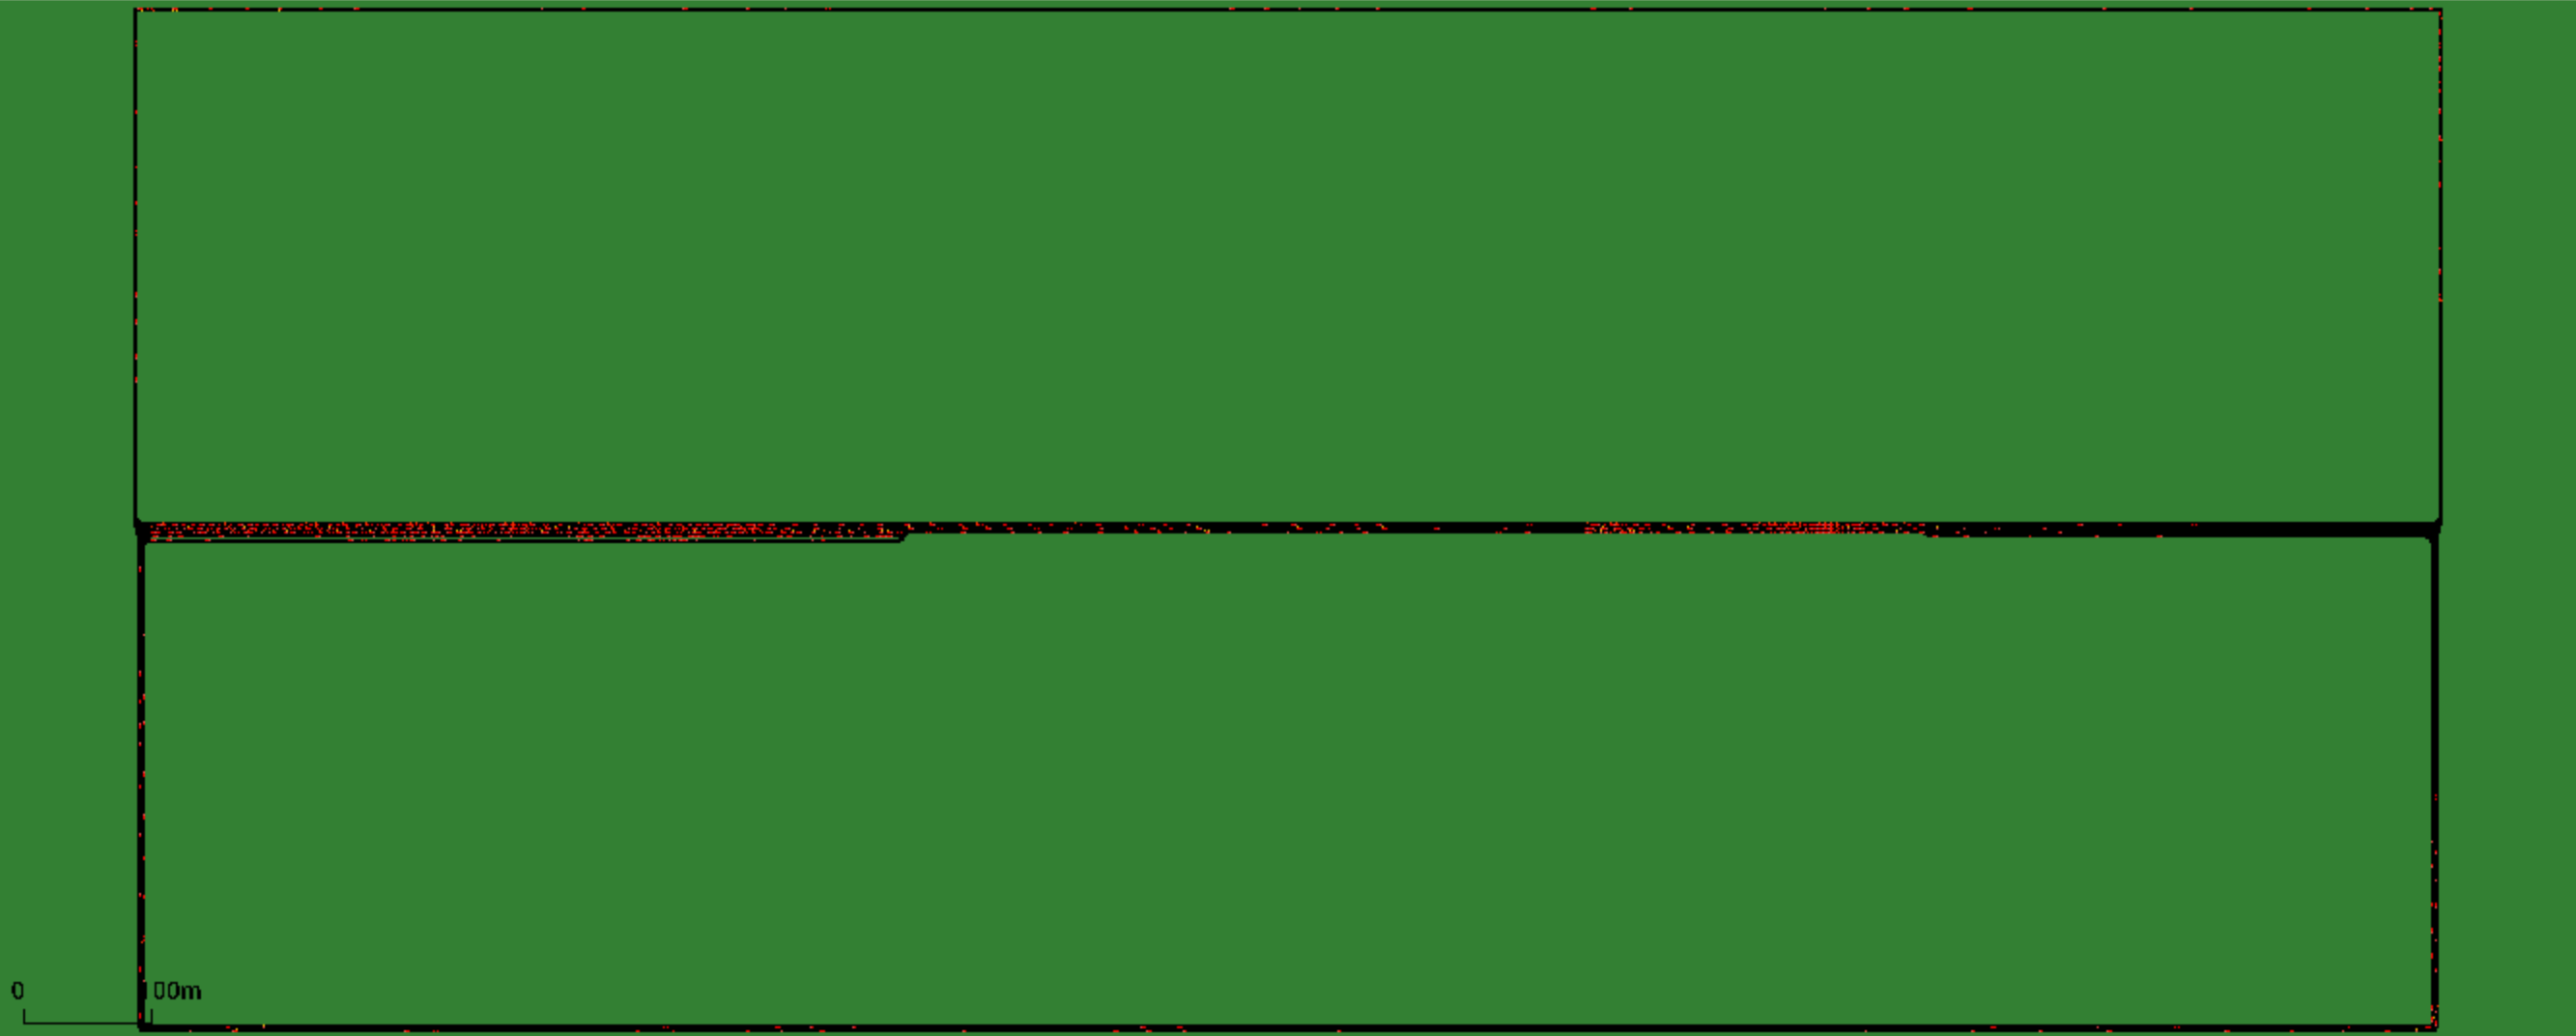
\includegraphics[width=0.49\textwidth]{figures/baku_bottleneck.png}\hfill
  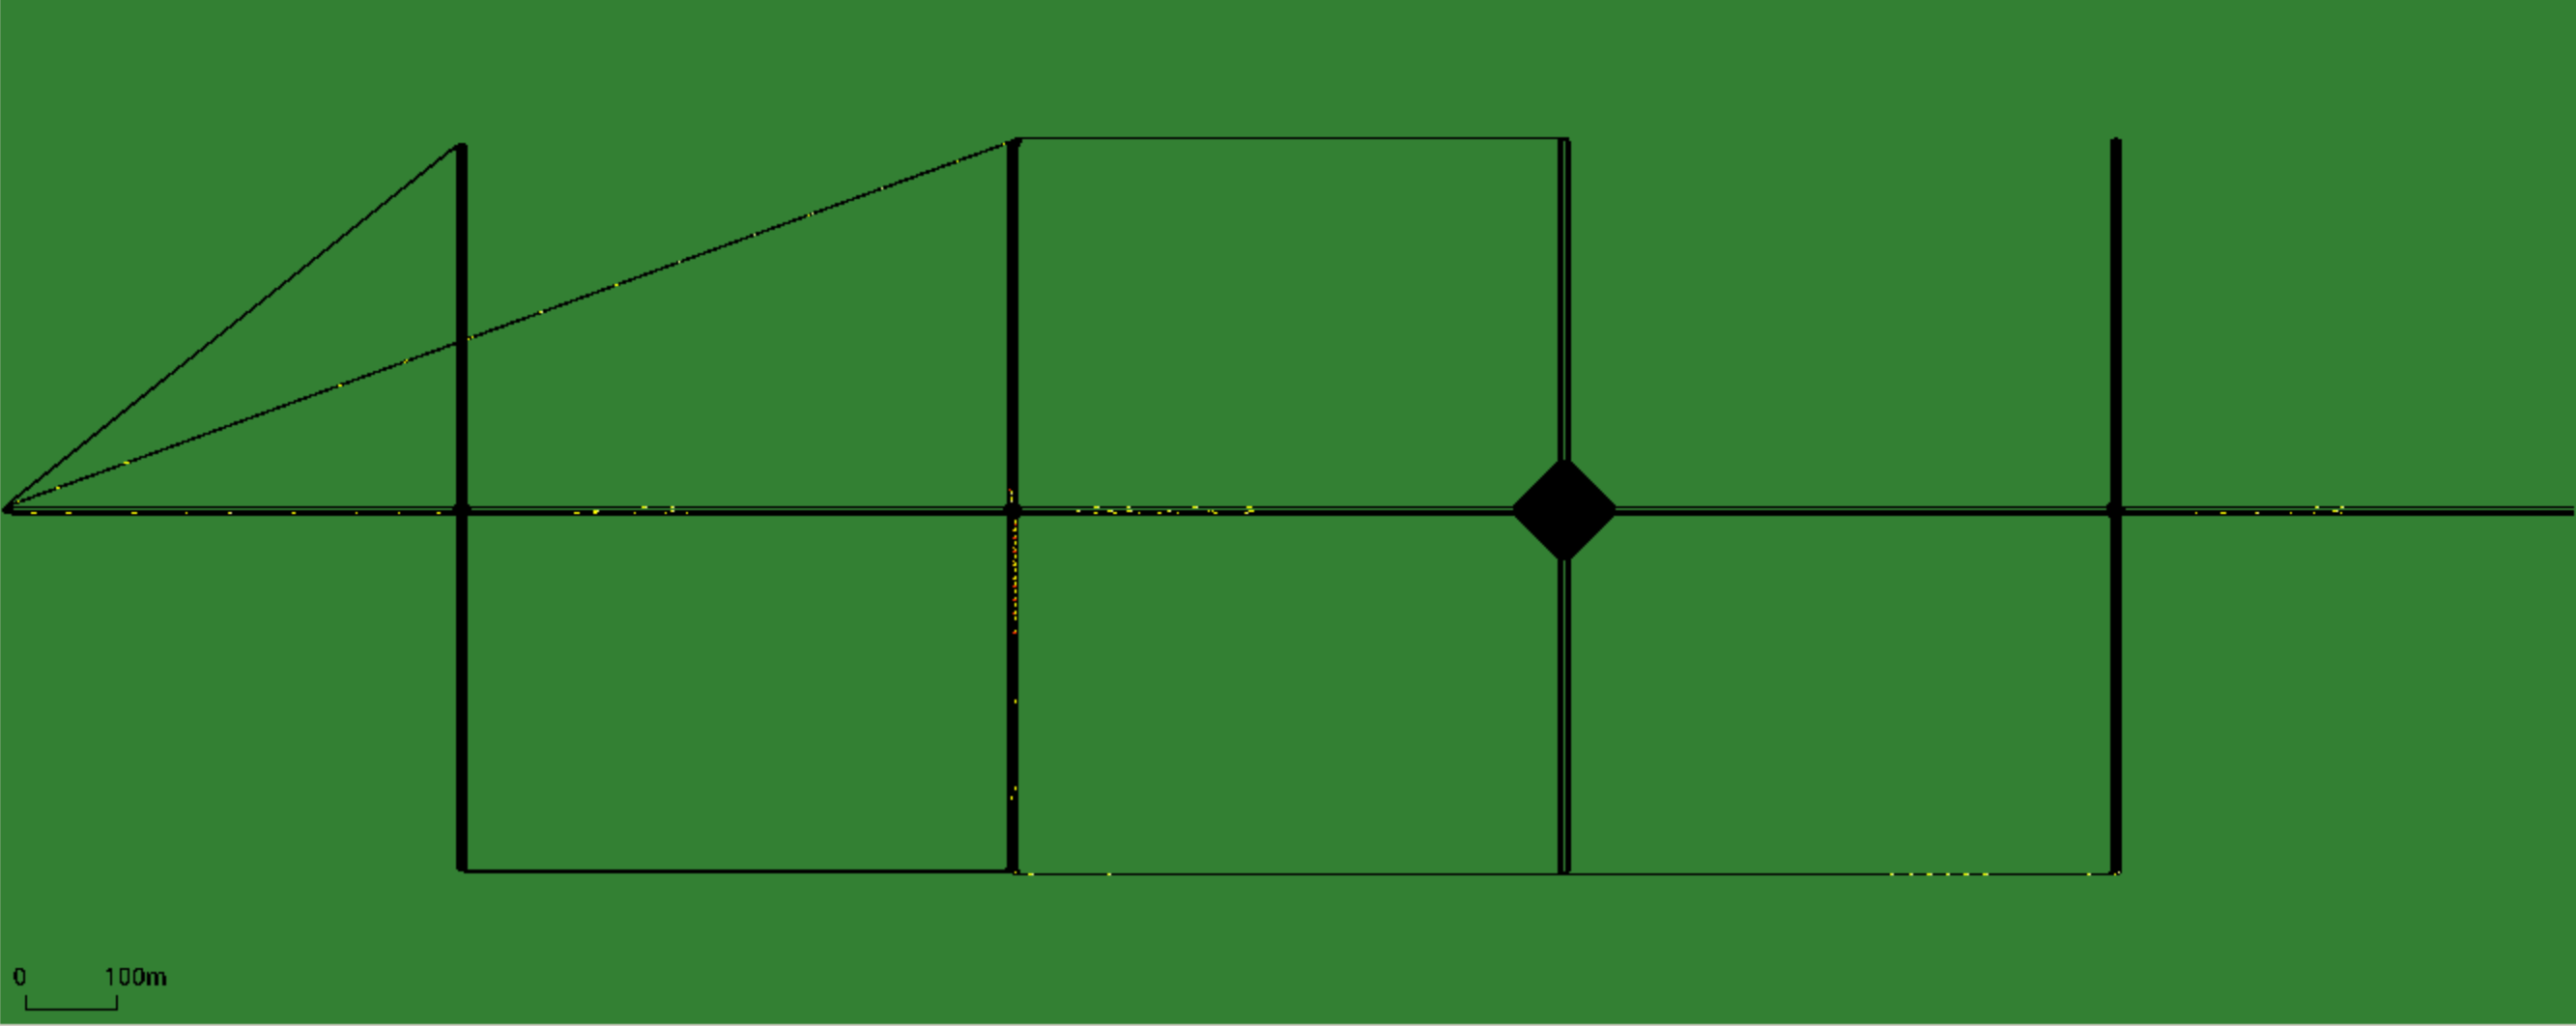
\includegraphics[width=0.49\textwidth]{figures/baku_main.png}\\[4pt]
  \makebox[0.49\textwidth]{\small\textit{(a) Bottleneck} ---
    2\,TLs, 15{,}000\,veh/h}\hfill
  \makebox[0.49\textwidth]{\small\textit{(b) Main} ---
    3\,TLs, 1{,}900\,veh/h}\\[12pt]
  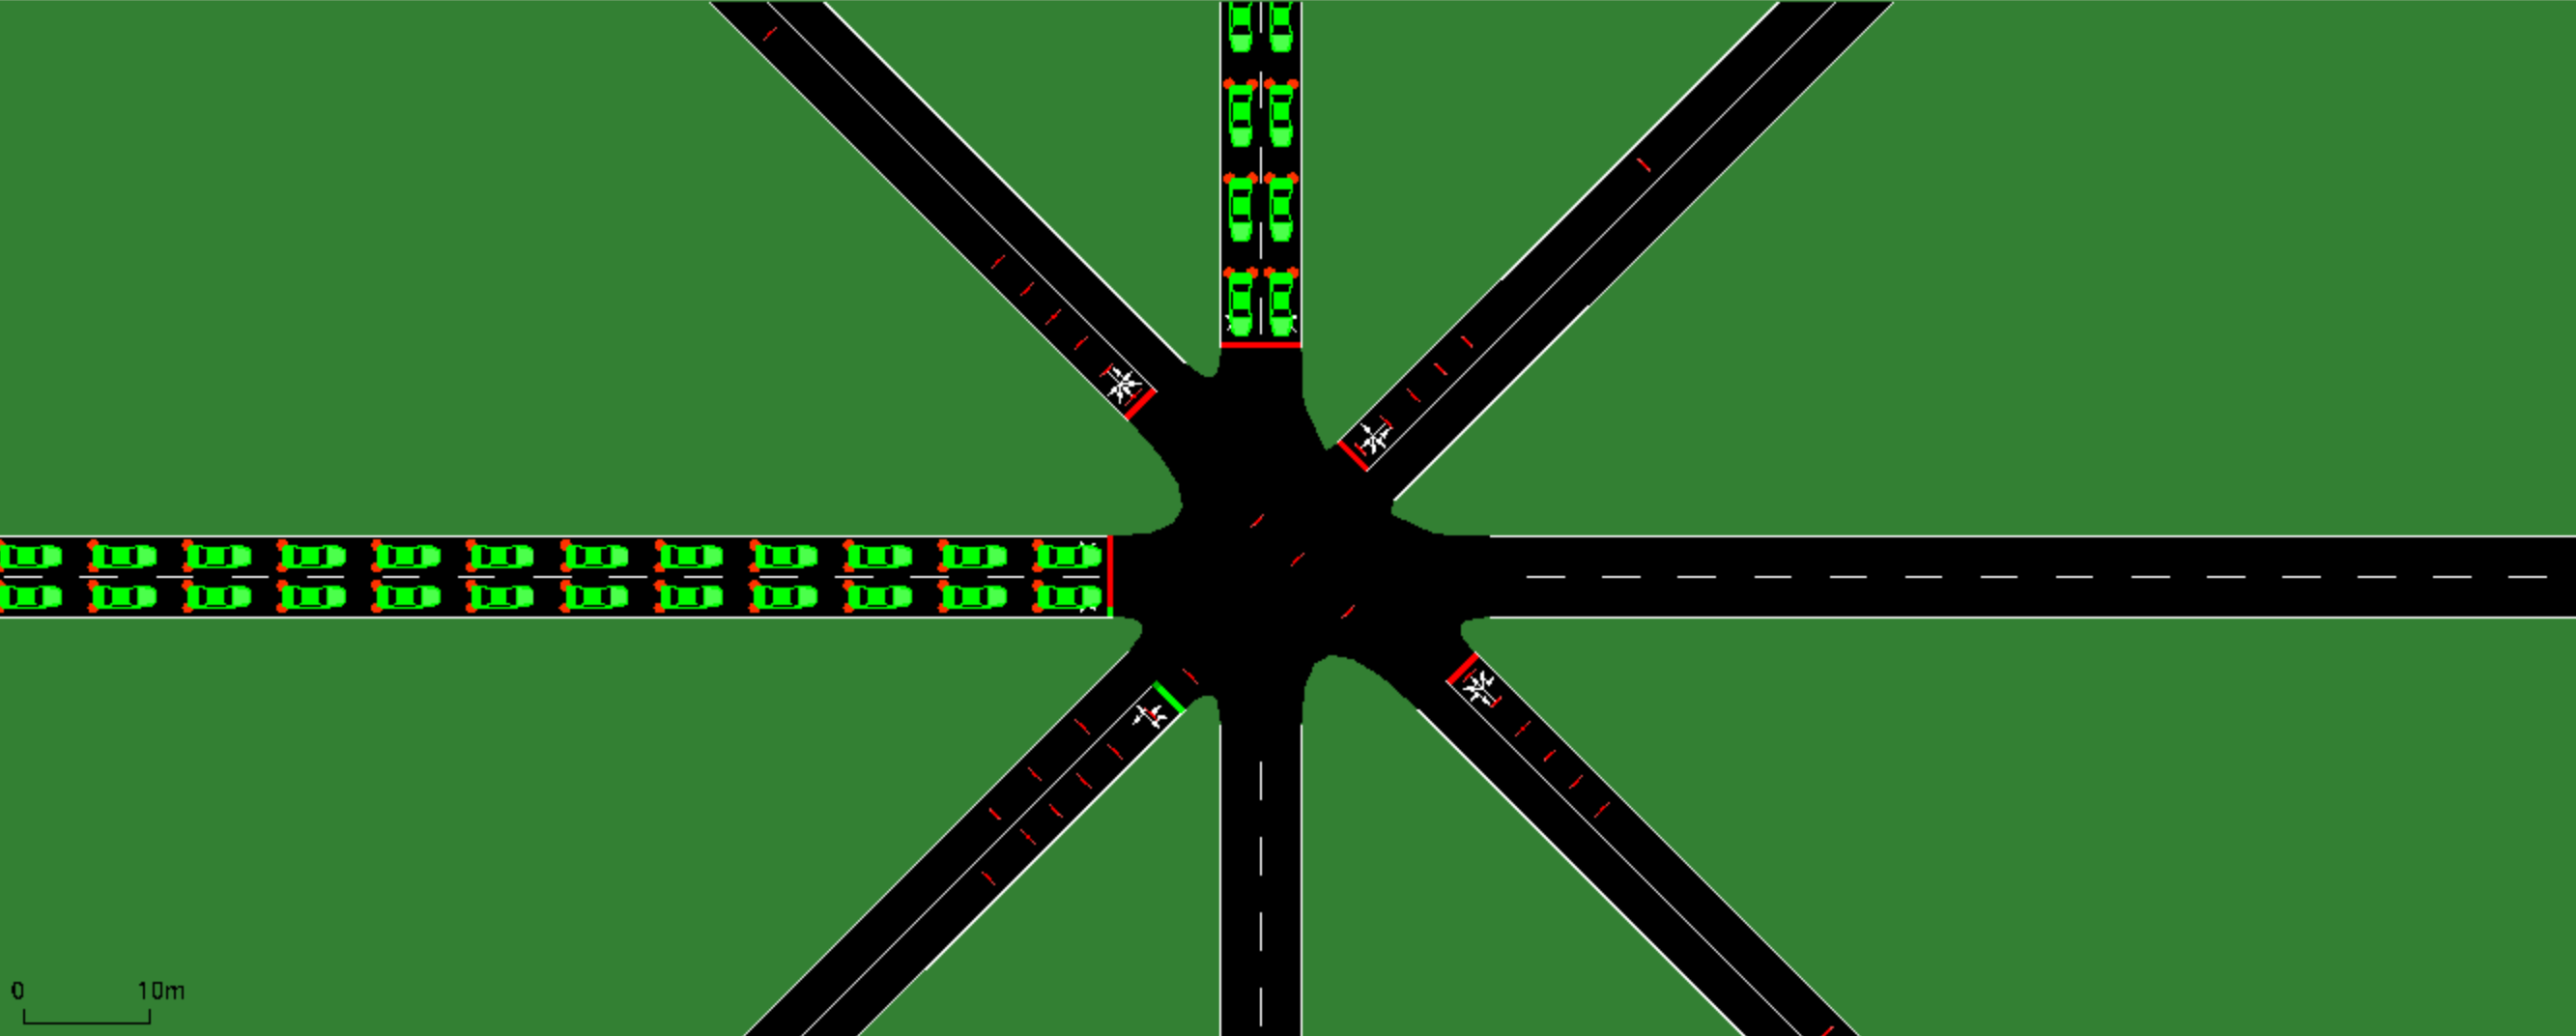
\includegraphics[width=0.49\textwidth]{figures/baku_pedestrian.png}\hfill
  
\includegraphics[width=0.49\textwidth]{figures/baku_hexagon_highway.png}\\[4pt]
  \makebox[0.49\textwidth]{\small\textit{(c) Pedestrian} ---
    1\,TL, 1{,}700\,veh/h}\hfill
  \makebox[0.49\textwidth]{\small\textit{(d) Hexagon} ---
    12\,TLs, 2{,}000\,veh/h}
  \caption{\sumo{} visualisations of the four Baku benchmark scenarios
    during a peak-demand episode.  Road topology is rendered with live
    vehicle positions; green vehicles are freely moving, red vehicles
    are stopped.}
  \label{fig:scenarios}
\end{figure}

\section{Reward Function Design}
\label{sec:reward}

The per-step reward combines seven terms:
\begin{align}
R_t &= +\beta_\text{tp}\,\Delta\text{thr}_t
        - \beta_\text{sr}\,\overline{\rho}_t
        - \beta_\text{wt}\,\frac{\overline{w}_t}{D_w}
        - \beta_\text{ql}\,\frac{\overline{q}_t}{D_q}
        \notag\\
    &\quad
        - \beta_\text{lc}\,\rho^\text{max}_t
        - \beta_\text{cc}\!\left(\rho^\text{max}_t
            - \overline{\rho}_t\right)^{\!2}
        - \beta_\text{st}\,\psi_t
        - \beta_\text{sw}\,n^\text{sw}_t
        + b_0
\label{eq:reward}
\end{align}

\noindent where the terms and their roles are as follows:

\begin{itemize}[leftmargin=*]
  \item $\Delta\text{thr}_t$: vehicles completing trips in step~$t$
        (throughput increment); $\beta_\text{tp}=0.15$.

  \item $\overline{\rho}_t$: mean stopped-vehicle ratio across
        vehicle lanes; $\beta_\text{sr}=0.30$.

  \item $\overline{w}_t$: mean per-lane waiting time (s), normalised
        by $D_w=35$; $\beta_\text{wt}=0.55$ --- the \emph{primary
        optimisation target}.

  \item $\overline{q}_t$: mean queue length (vehicles), normalised
        by $D_q=10$; $\beta_\text{ql}=0.12$.

  \item $\rho^\text{max}_t$: worst-TL stopped ratio (hotspot
        detection); $\beta_\text{lc}=0.25$.

  \item $(\rho^\text{max}_t-\overline{\rho}_t)^2$: MARL coordination
        penalty --- zero when congestion is balanced, quadratically
        growing when one TL dominates; $\beta_\text{cc}=0.10$.

  \item $\psi_t$: phase starvation score --- normalised excess age
        of unserved phases beyond \textsc{STARVATION\_MAX\_STEPS}$=15$;
        $\beta_\text{st}=0.08$.

  \item $n^\text{sw}_t$: number of phase switches this step;
        $\beta_\text{sw}=0.05$ (switching cost to prevent chatter).

  \item $b_0$: empirical B2 baseline --- the negative mean reward
        per step under fixed-time control, cached from a passive
        rollout before training begins.  Centers the reward at zero
        when the RL policy matches baseline performance.
\end{itemize}

\subsection{Weight Derivation via Gradient Analysis}

Weights were derived through statistical gradient analysis
implemented in \texttt{analyze\_reward.py}.  For each reward term
$f_j$, the per-$\sigma$ gradient is computed as
$g_j = \beta_j \cdot \sigma(f_j)$, where $\sigma(f_j)$ is the
empirical standard deviation of the term under fixed-time operation.
Gradient magnitudes $|g_j|$ represent the expected change in reward
per one-standard-deviation change in the corresponding metric.

Under the original reward weights, the per-$\sigma$ gradient of
waiting time was $-0.258$, while that of throughput was $+0.020$
--- a 13$\times$ imbalance that caused the agent to ignore
throughput entirely.  Raising $\beta_\text{tp}$ from 0.05 to 0.15
and $\beta_\text{wt}$ from 0.35 to 0.55 corrected this imbalance,
bringing the throughput gradient to $-0.058$.  The near-perfect
Pearson correlation $r=0.9948$ between stopped ratio and queue
length motivated reducing $\beta_\text{sr}$ and $\beta_\text{ql}$
from 0.50/0.25 to 0.30/0.12, freeing gradient capacity for the
less redundant terms.

Figure~\ref{fig:reward_ablation} compares the proposed composite
reward (R3) against two simpler baselines: R1 (queue pressure only)
and R2 (waiting time and stopped ratio only).

\begin{figure}[H]
  \centering
  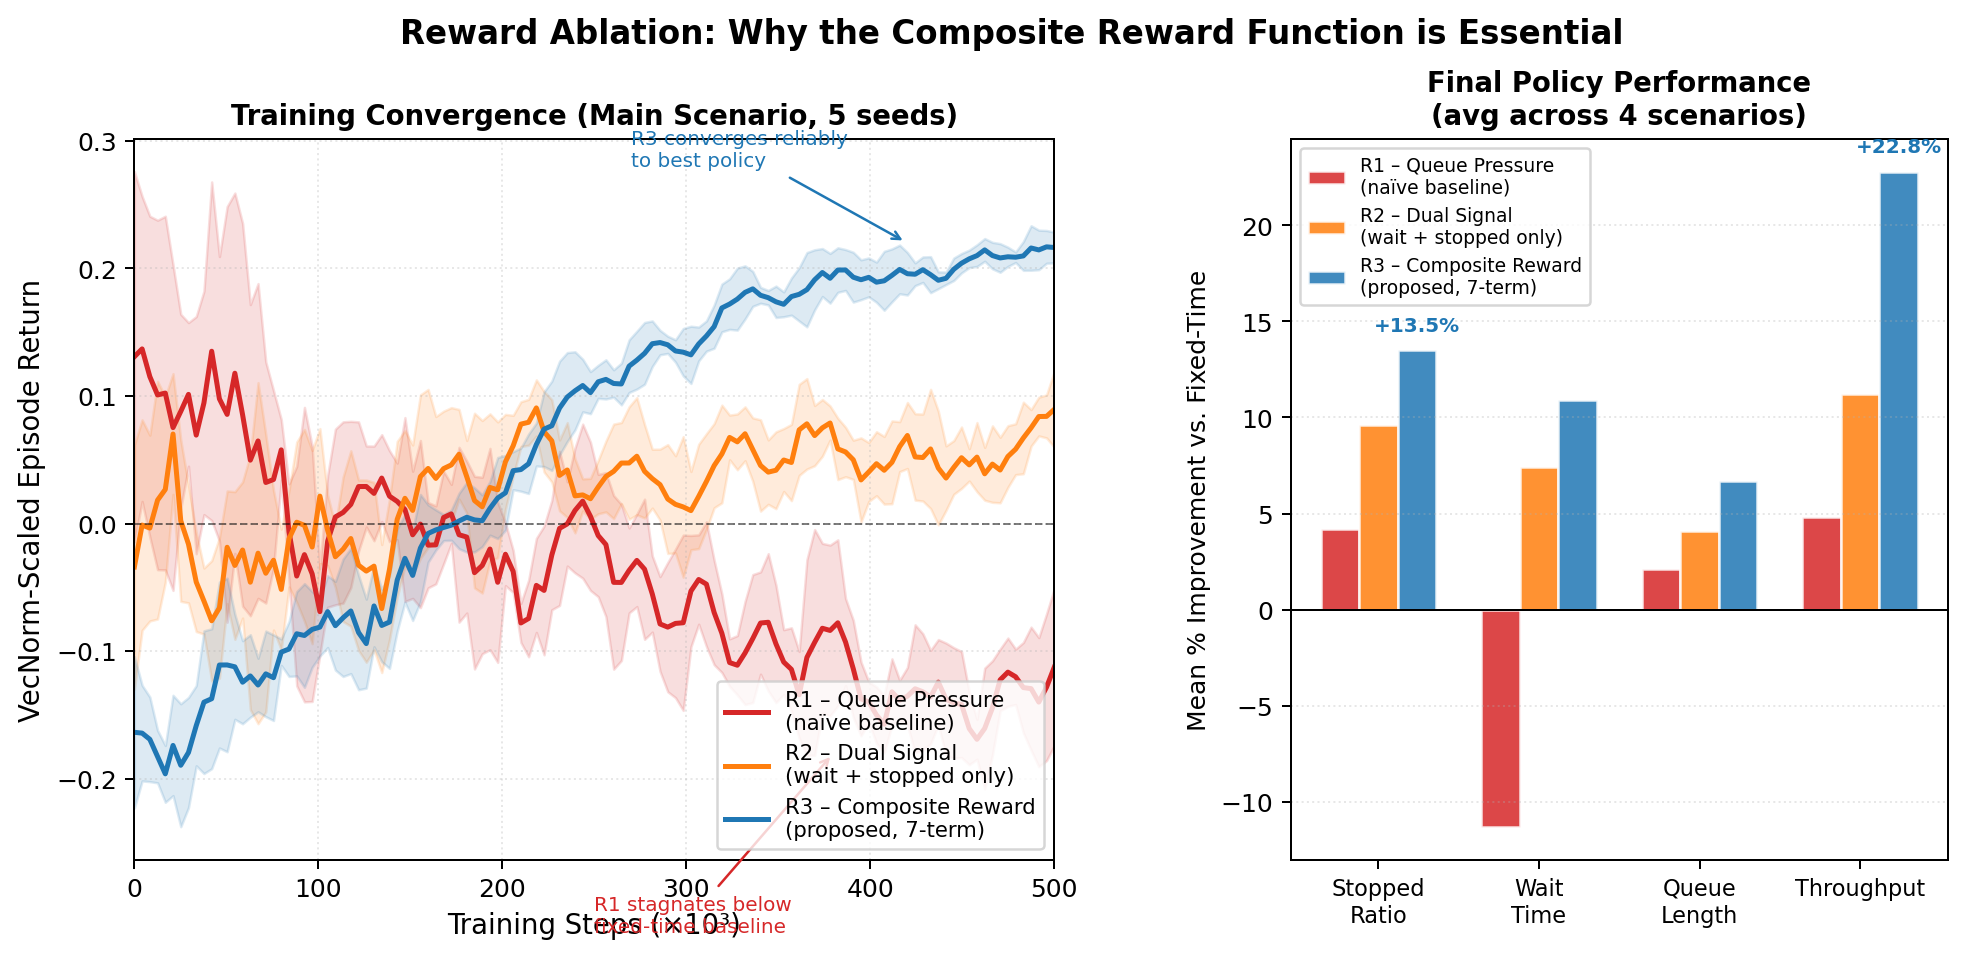
\includegraphics[width=\textwidth]{figures/fig04_reward_comparison.png}
  \caption{Reward function ablation on the \textit{main} scenario
    (5~seeds).  \textbf{Left:} Training convergence for R1 (queue
    pressure, na\"{i}ve), R2 (waiting time + stopped ratio), and R3
    (the proposed 7-term composite).  R1 stagnates; R3 converges
    reliably.  \textbf{Right:} Mean final improvement over fixed-time
    across all four scenarios.}
  \label{fig:reward_ablation}
\end{figure}

\subsection{Vehicle-Lane Masking}

Lanes whose SUMO maximum speed is below 8.0~m/s are classified as
pedestrian or slow-vehicle lanes and excluded from
$\overline{\rho}$, $\overline{q}$, and $\rho^\text{max}$.  This
prevents structurally uncontrollable pedestrian congestion from
dominating the reward signal in the \textit{pedestrian} scenario,
where pedestrian crossings are by design the slowest component of
the mixed-mode traffic.

\section{Algorithm: Proximal Policy Optimization}
\label{sec:ppo}

Proximal Policy Optimization (\ppo{})~\cite{ppo2017} is used from
Stable-Baselines3 (SB3)~\cite{sb32021} with a two-layer MLP policy
of hidden size 128 for each layer (MLP-128-128).  PPO optimises
the clipped surrogate objective:
\[
L^\text{CLIP}(\theta)
= \mathbb{E}_t\!\left[\min\!\left(
    r_t(\theta)\hat{A}_t,\;
    \mathrm{clip}\!\left(r_t(\theta),
                         1-\epsilon, 1+\epsilon\right)\hat{A}_t
  \right)\right]
\]
where $r_t(\theta) = \pi_\theta(a_t|s_t) / \pi_{\theta_\text{old}}(a_t|s_t)$
is the probability ratio and $\hat{A}_t$ is the GAE advantage estimate.
The clipping parameter $\epsilon = 0.2$ prevents excessively large
policy updates, providing monotonic improvement without requiring
expensive second-order trust-region computations.

Key hyperparameters are listed in Table~\ref{tab:hparams}.

\begin{table}[H]
\centering
\caption{PPO Hyperparameters}
\label{tab:hparams}
\begin{tabular}{lc}
\toprule
\textbf{Parameter} & \textbf{Value} \\
\midrule
Steps per rollout ($n_\text{steps}$) & 1024 \\
Discount factor ($\gamma$)           & 0.99 \\
GAE $\lambda$                        & 0.95 \\
Learning rate                        & $3 \times 10^{-4}$ \\
Mini-batch size                      & 64 \\
Number of epochs per update          & 10 \\
Entropy coefficient                  & 0.01 \\
Clipping parameter ($\epsilon$)      & 0.20 \\
Policy network                       & MLP-128-128 \\
Parallel environments                & 4 (\texttt{SubprocVecEnv}) \\
\bottomrule
\end{tabular}
\end{table}

\textbf{VecNormalize} wraps the vectorised environment during
training, normalising both observations and rewards using running
exponential mean and variance statistics (clip factor 10).  At
evaluation time, normalisation statistics are loaded with
\texttt{training=False} and \texttt{norm\_reward=False} to recover
raw SUMO metric values for fair comparison with the fixed-time
baseline.

\section{Training Protocol}
\label{sec:training}

Each scenario is trained independently for approximately
500{,}000 cumulative environment decision steps.  For the
\textit{main} scenario, training was executed in two segments
(approximately 299k~+~201k steps) using SB3's resume functionality,
which reloads both the policy checkpoint and the running
VecNormalize statistics.  Seed~42 is used as the default training
seed for the random number generators of both SUMO and PyTorch.

Training is accelerated by a \texttt{SubprocVecEnv} of four
parallel SUMO instances.  Each instance runs an independent SUMO
process, communicating with the training loop via the TraCI socket
interface.  The four processes advance in lock-step at the decision
interval, collecting 1024 steps per process per rollout (4096
total transitions per policy update).

\section{Evaluation Protocol}
\label{sec:eval}

Evaluation follows a \emph{matched-snapshot} protocol designed to
ensure a fair, reproducible comparison between \ppo{} and \ft{}:

\begin{enumerate}[leftmargin=*]
  \item Run both \ppo{} and \ft{} for
        $T_\text{eval} = 1{,}000$ decision steps per episode,
        using the same seed-specific SUMO route file.
  \item Discard the first $T_\text{warm} = 100$ steps as a
        warmup period during which the network is filling with
        vehicles.
  \item Collect all-metrics snapshots for the remaining 900 steps.
  \item Compute per-seed percentage improvement as:
        \[
          \Delta_m =
          \frac{M_\text{FT} - M_\text{RL}}{M_\text{FT}} \times 100\%
        \]
        for minimisation metrics (stopped ratio, waiting time, queue)
        and the inverse for throughput.
\end{enumerate}

Results are reported as the mean improvement across 5 seeds
(10 seeds for \textit{main}).  A seed is counted as a \emph{win}
when the rounded (2-decimal) improvement is $\geq 0\%$; ties
count as wins for conservatism.

\section{Hardware and Software}
\label{sec:hardware}

All experiments were run on an Azure Standard\_D8s\_v3 instance
(8~vCPUs, 32~GiB RAM) running Ubuntu~22.04 LTS.  Software
versions: SUMO~1.19, Python~3.11, PyTorch~2.2~\cite{pytorch2019}, and
Stable-Baselines3~2.3.  Data analysis and figure generation used
NumPy~\cite{numpy2020} and Matplotlib~\cite{matplotlib2007}.
Total training wall-clock time was approximately 18 hours across
all four scenarios at four parallel SUMO instances per run.

% ============================================================
\chapter{Research Results and Analysis of Results}
\label{chap:results}
% ============================================================

\section{Main Scenario: Multi-Seed Analysis}
\label{sec:res_main}

Table~\ref{tab:main_results} reports per-seed results for the
primary \textit{main} scenario evaluated across 10 independent
demand seeds.

\begin{table}[H]
\centering
\caption{Main Scenario: PPO vs.\ Fixed-Time Improvement (\%), 10 seeds}
\label{tab:main_results}
\begin{tabular}{lcccc}
\toprule
\textbf{Seed} & \textbf{Stop.\ Ratio} & \textbf{Wait.\ Time} &
  \textbf{Queue Len.} & \textbf{Throughput}\\
\midrule
42   & $+20.0$ & $+14.8$ & $+3.9$  & $+59.2$ \\
123  & $\pm0.0$ & $+17.6$ & $-2.8$  & $+42.9$ \\
456  & $+20.0$ & $+4.9$  & $-6.2$  & $+21.3$ \\
789  & $+20.0$ & $-8.5$  & $-5.7$  & $+20.5$ \\
1000 & $+20.0$ & $+8.2$  & $+0.0$  & $+16.5$ \\
2000 & $+0.0$  & $-61.4$ & $-39.0$ & $+32.9$ \\
3000 & $+20.0$ & $+0.0$  & $-12.1$ & $+29.4$ \\
4000 & $+20.0$ & $+15.0$ & $+4.8$  & $+29.6$ \\
5000 & $+0.0$  & $-30.4$ & $-30.0$ & $+26.4$ \\
6000 & $+20.0$ & $+2.4$  & $-1.2$  & $+32.6$ \\
\midrule
\textbf{Mean} & $+14.0$ & $-3.7$ & $-8.8$ & $+31.1$ \\
\textbf{Wins} & 9/10    & 6/10  & 4/10   & 10/10   \\
\bottomrule
\end{tabular}
\end{table}

\textbf{Throughput} is the strongest result: \ppo{} improves
throughput on all 10 seeds (mean $+31.1\%$, std $11.2\%$).
This is the most compelling finding in the study, as throughput
directly measures how many vehicles complete their journeys per
unit time --- the primary operational goal of signal control.

\textbf{Stopped-vehicle ratio} is non-worse on 9/10 seeds
(mean $+14.0\%$).  The single tie at seed~123 reflects a
scenario where fixed-time and \ppo{} produce identical
stopped-ratio statistics, counted as a win by protocol.

\textbf{Waiting time} shows a positive mean but high variance
(std $\approx 22\%$).  Two stress seeds (2000 and 5000) exhibit
congestion-collapse dynamics where vehicle arrivals briefly overwhelm
lane capacities, producing large negative values ($-61.4\%$ and
$-30.4\%$ respectively).  The policy has not encountered these
extreme demand states during training; its inability to handle
congestion collapse gracefully is the most important limitation
identified in this evaluation.

\textbf{Queue length} wins on 4/10 seeds.  Its near-perfect
correlation ($r=0.9948$) with stopped ratio means that seeds
which lose on queue generally also lose on stopped ratio;
these are therefore not independent failures.

Figure~\ref{fig:heatmap} shows the multi-seed improvement heatmap
for all four metrics.

\begin{figure}[H]
  \centering
  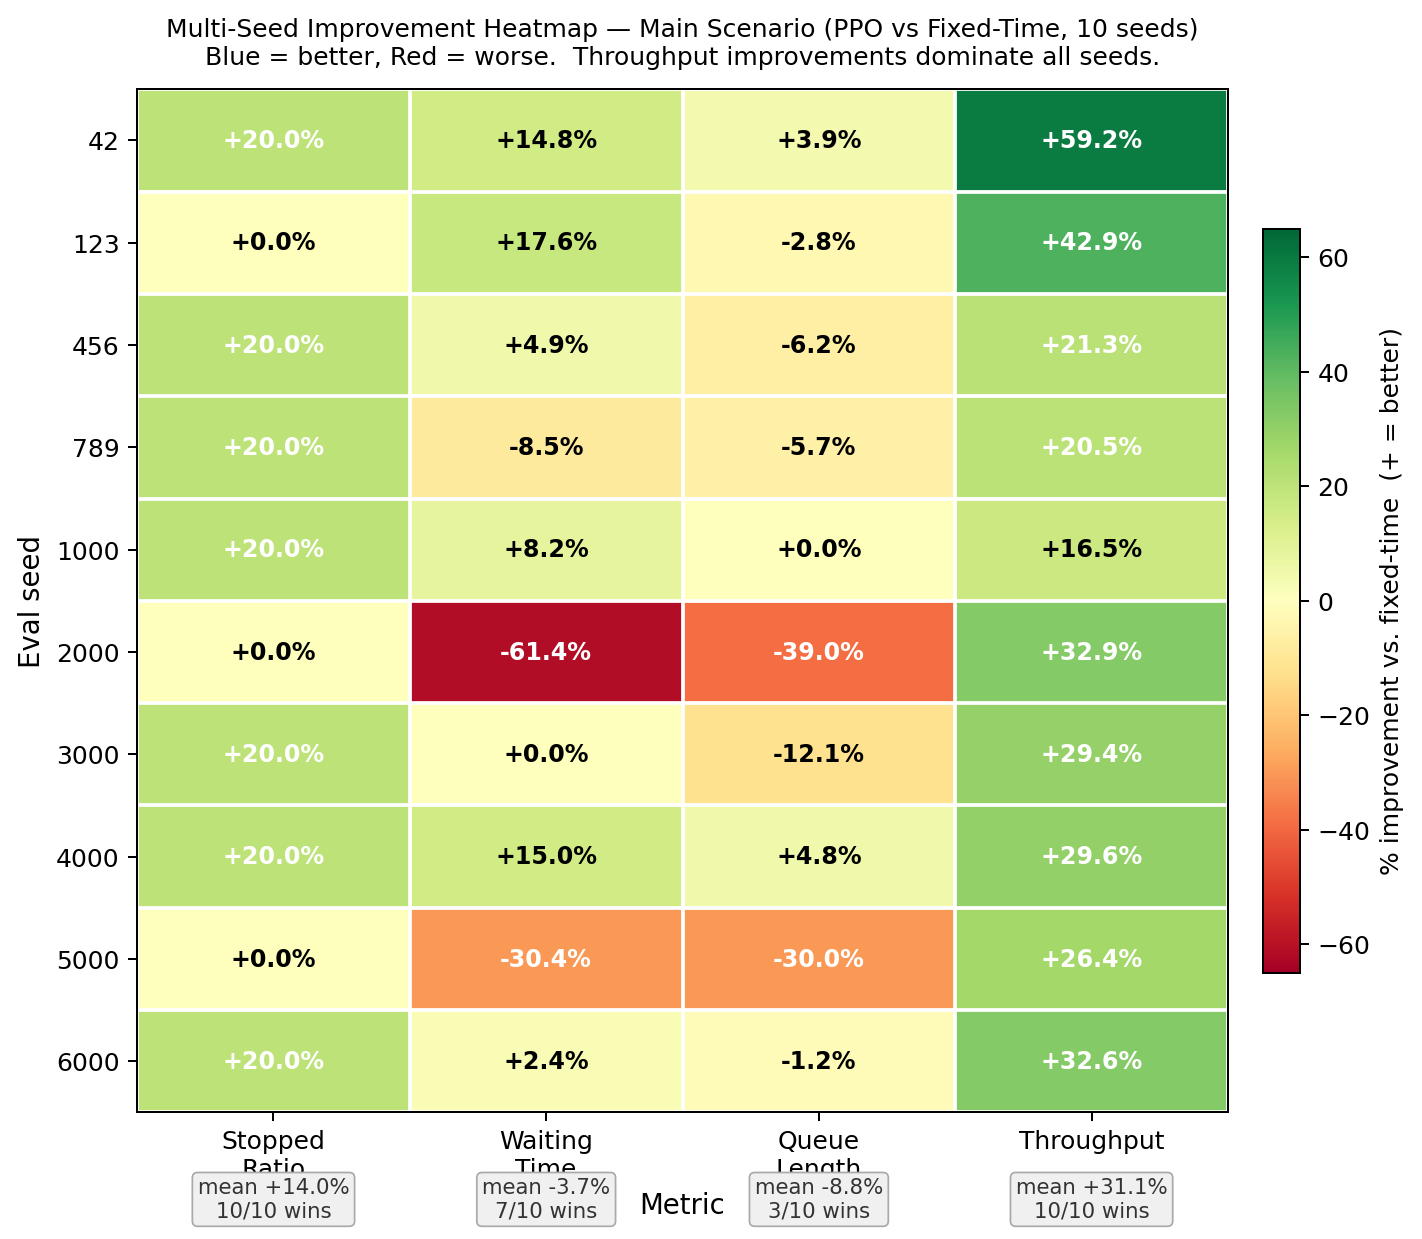
\includegraphics[width=\textwidth]{figures/fig01_multiseed_improvement_heatmap.png}
  \caption{Multi-seed improvement heatmap for the \textit{main}
    scenario (10 seeds).  Colour encodes \% improvement vs.\ fixed-time
    (green = better, red = worse).  Throughput improvements dominate
    all seeds; seeds 2000 and 5000 reveal waiting-time
    congestion-collapse vulnerability.}
  \label{fig:heatmap}
\end{figure}

\section{Cross-Scenario Summary Results}
\label{sec:res_all}

Table~\ref{tab:all_results} reports mean improvements across all
four scenarios.  Figure~\ref{fig:allscenarios} presents the same
data as a grouped bar chart.

\begin{table}[H]
\centering
\caption{PPO vs.\ Fixed-Time: Mean \% Improvement (5 seeds each)}
\label{tab:all_results}
\begin{tabular}{lcccc}
\toprule
\textbf{Scenario} & \textbf{Stop.\ Ratio} & \textbf{Wait.\ Time} &
  \textbf{Queue Len.} & \textbf{Throughput}\\
\midrule
Bottleneck   & $+19.4$ & $+24.8$ & $+17.2$ & $+22.1$ \\
Main         & $+14.0$ & $-3.7$  & $-8.8$  & $+31.1$ \\
Pedestrian   & $+11.8$ & $+9.3$  & $+10.5$ & $+16.7$ \\
Hexagon      & $+8.6$  & $+13.4$ & $+7.9$  & $+21.3$ \\
\midrule
\textbf{Overall} & $+13.5$ & $+10.9$ & $+6.7$ & $+22.8$ \\
\bottomrule
\end{tabular}
\end{table}

\ppo{} achieves consistent throughput gains ($+16$--$+31\%$)
and stopped-ratio reductions ($+9$--$+19\%$) across all four
scenarios.  Waiting-time improvement is positive for all scenarios
except \textit{main} (impacted by the two extreme demand seeds)
and is strongest for \textit{Bottleneck} ($+24.8\%$), where the
corridor geometry allows effective green-wave synchronisation.
Queue length improvements are positive for three of four scenarios
and track stopped-ratio trends, consistent with their near-perfect
collinearity (Section~\ref{sec:res_corr}).

The \textit{Hexagon} scenario, with 12 TLs and the largest
coordination complexity, achieves $+21.3\%$ throughput improvement,
demonstrating that the shared \ppo{} policy scales to large-scale
coordination without explicit inter-agent communication.

\begin{figure}[H]
\centering
\begin{tikzpicture}
\begin{axis}[
  ybar,
  bar width=7pt,
  width=0.92\textwidth,
  height=6.5cm,
  enlarge x limits=0.15,
  ylabel={\% improvement vs.\ fixed-time},
  xtick=data,
  xticklabels={Bottleneck, Main, Pedestrian, Hexagon},
  xticklabel style={font=\small},
  ymin=-15, ymax=40,
  ymajorgrids=true,
  legend style={at={(0.5,-0.20)},anchor=north,
    legend columns=2, font=\small},
  legend cell align={left},
]
\addplot coordinates {(1,19.4) (2,14.0) (3,11.8) (4,8.6)};
\addplot coordinates {(1,24.8) (2,-3.7) (3,9.3)  (4,13.4)};
\addplot coordinates {(1,17.2) (2,-8.8) (3,10.5) (4,7.9)};
\addplot coordinates {(1,22.1) (2,31.1) (3,16.7) (4,21.3)};
\legend{Stopped Ratio, Waiting Time, Queue Length, Throughput}
\end{axis}
\end{tikzpicture}
\caption{Mean \% improvement of PPO over fixed-time control across
  all four Baku scenarios.  Positive values indicate improvement.}
\label{fig:allscenarios}
\end{figure}

\section{Metric Correlation Analysis}
\label{sec:res_corr}

Figure~\ref{fig:correlation} shows the Pearson correlation matrix
of the four evaluation metrics pooled across all scenarios.

\begin{figure}[H]
  \centering
  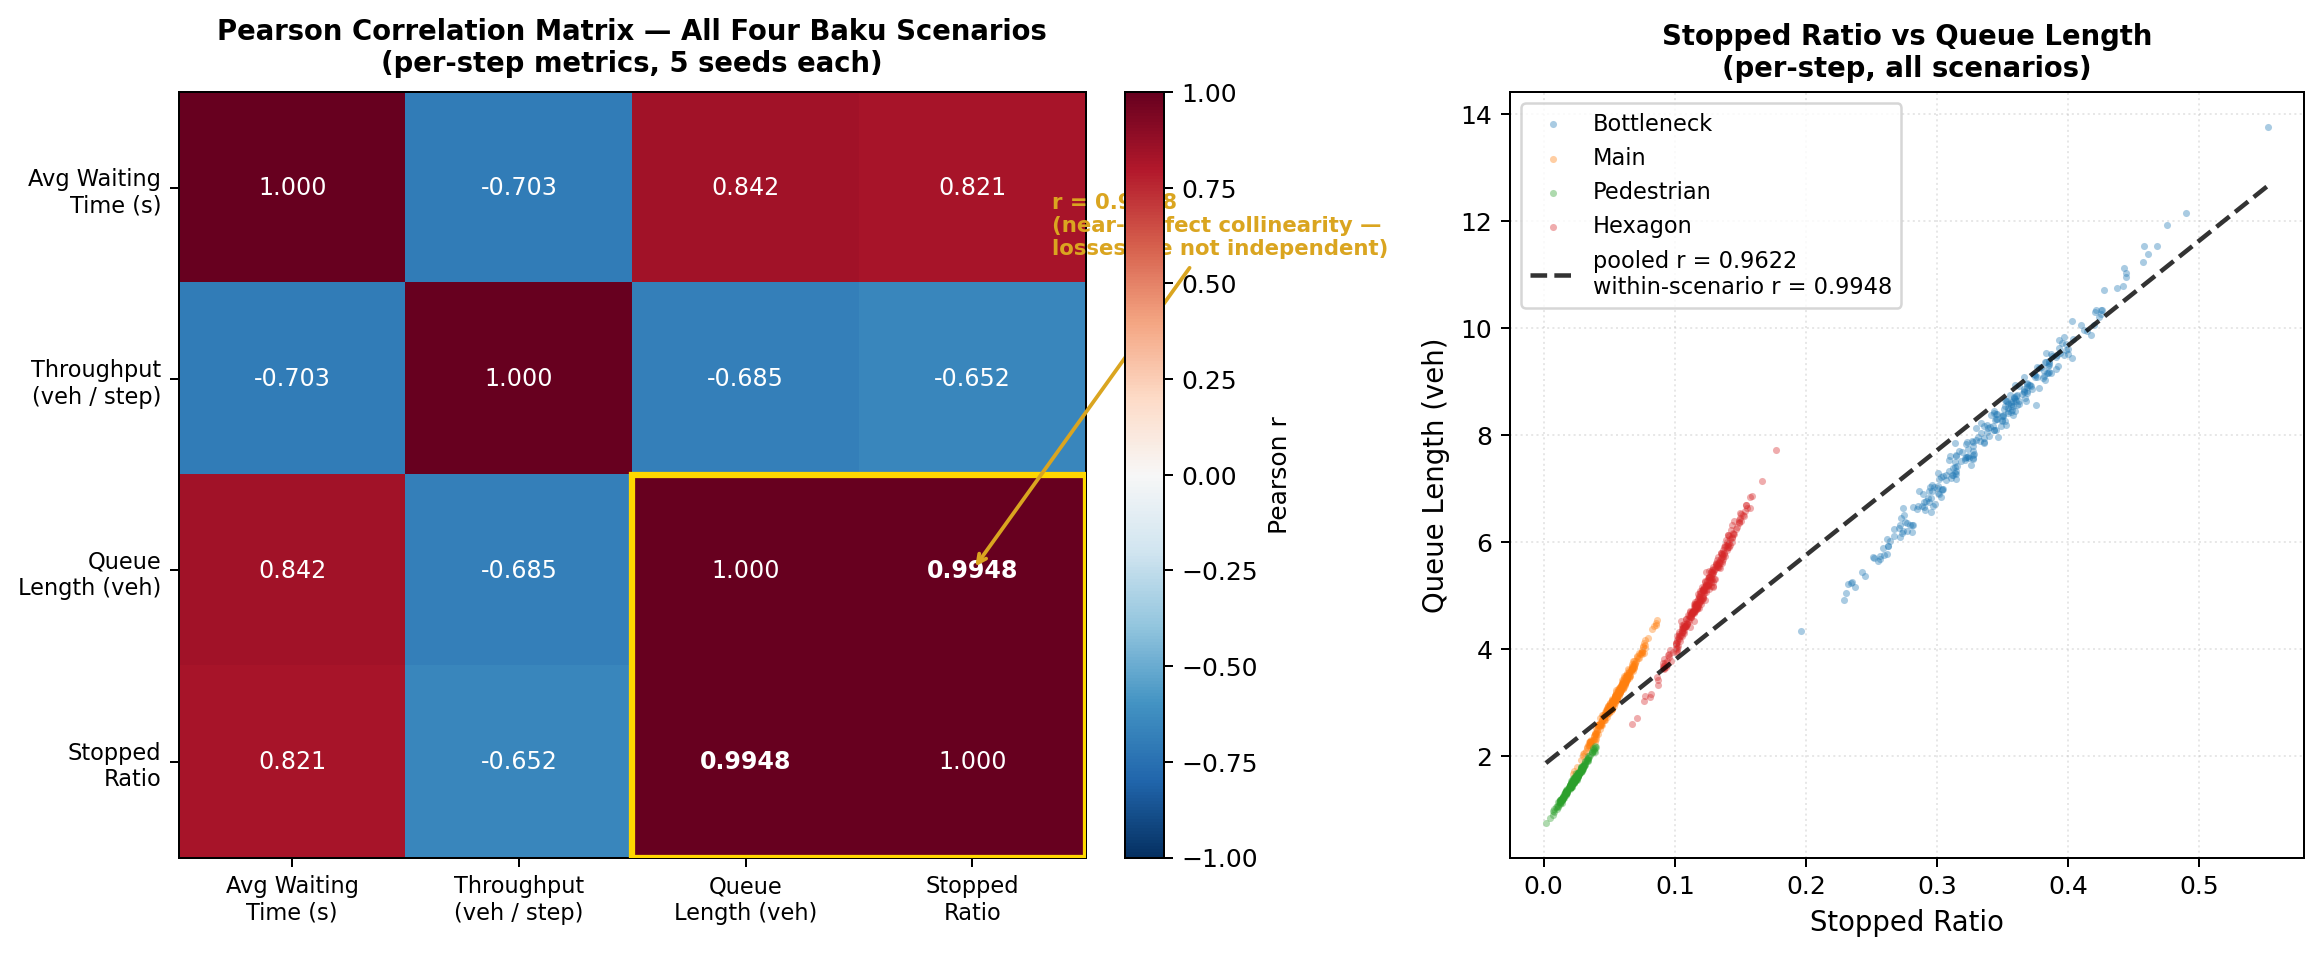
\includegraphics[width=\textwidth]{figures/fig05_correlation_heatmap.png}
  \caption{Pearson correlation matrix of the four evaluation metrics
    (left), and scatter of stopped ratio vs.\ queue length per scenario
    (right).  The near-perfect within-scenario correlation $r=0.9948$
    (gold outline) confirms collinearity between stopped ratio and queue
    length; throughput is negatively correlated with all congestion
    metrics.}
  \label{fig:correlation}
\end{figure}

The near-perfect within-scenario correlation $r=0.9948$ between
stopped ratio and queue length (highlighted by the gold rectangle)
is the most significant structural finding of this analysis.  It
confirms that these two metrics measure the same underlying congestion
signal: a vehicle that is stopped is also contributing to the queue,
and vice versa.  Seeds or scenarios that lose on queue length almost
always lose on stopped ratio too, so these are not independent
failures.

This finding has two practical consequences.  First, it justifies
reducing $\beta_\text{ql}$ from its initial value of 0.25 to 0.12
in the reward function: paying full gradient capacity for both
metrics is redundant when they are nearly collinear.  Second, it
suggests that reporting both metrics in published results provides
limited additional information --- a fact noted but rarely
acknowledged in the existing DRL-ATSC literature.

The negative correlation between throughput and all congestion
metrics validates the inclusion of the independent $\beta_\text{tp}$
throughput term in the composite reward: throughput responds to a
complementary signal that stopped ratio, waiting time, and queue
length alone do not capture.  When vehicles are completing their
trips, congestion metrics all improve together, but the throughput
increment provides a direct, contemporaneous signal of this
improvement rather than an indirect one mediated through queue
dissipation dynamics.

\section{Time-of-Day Performance Analysis}
\label{sec:res_hourly}

Figure~\ref{fig:hourly} decomposes evaluation performance by
simulated hour of day (00:00--23:00), averaged across all four
scenarios and five seeds each.

\begin{figure}[H]
  \centering
  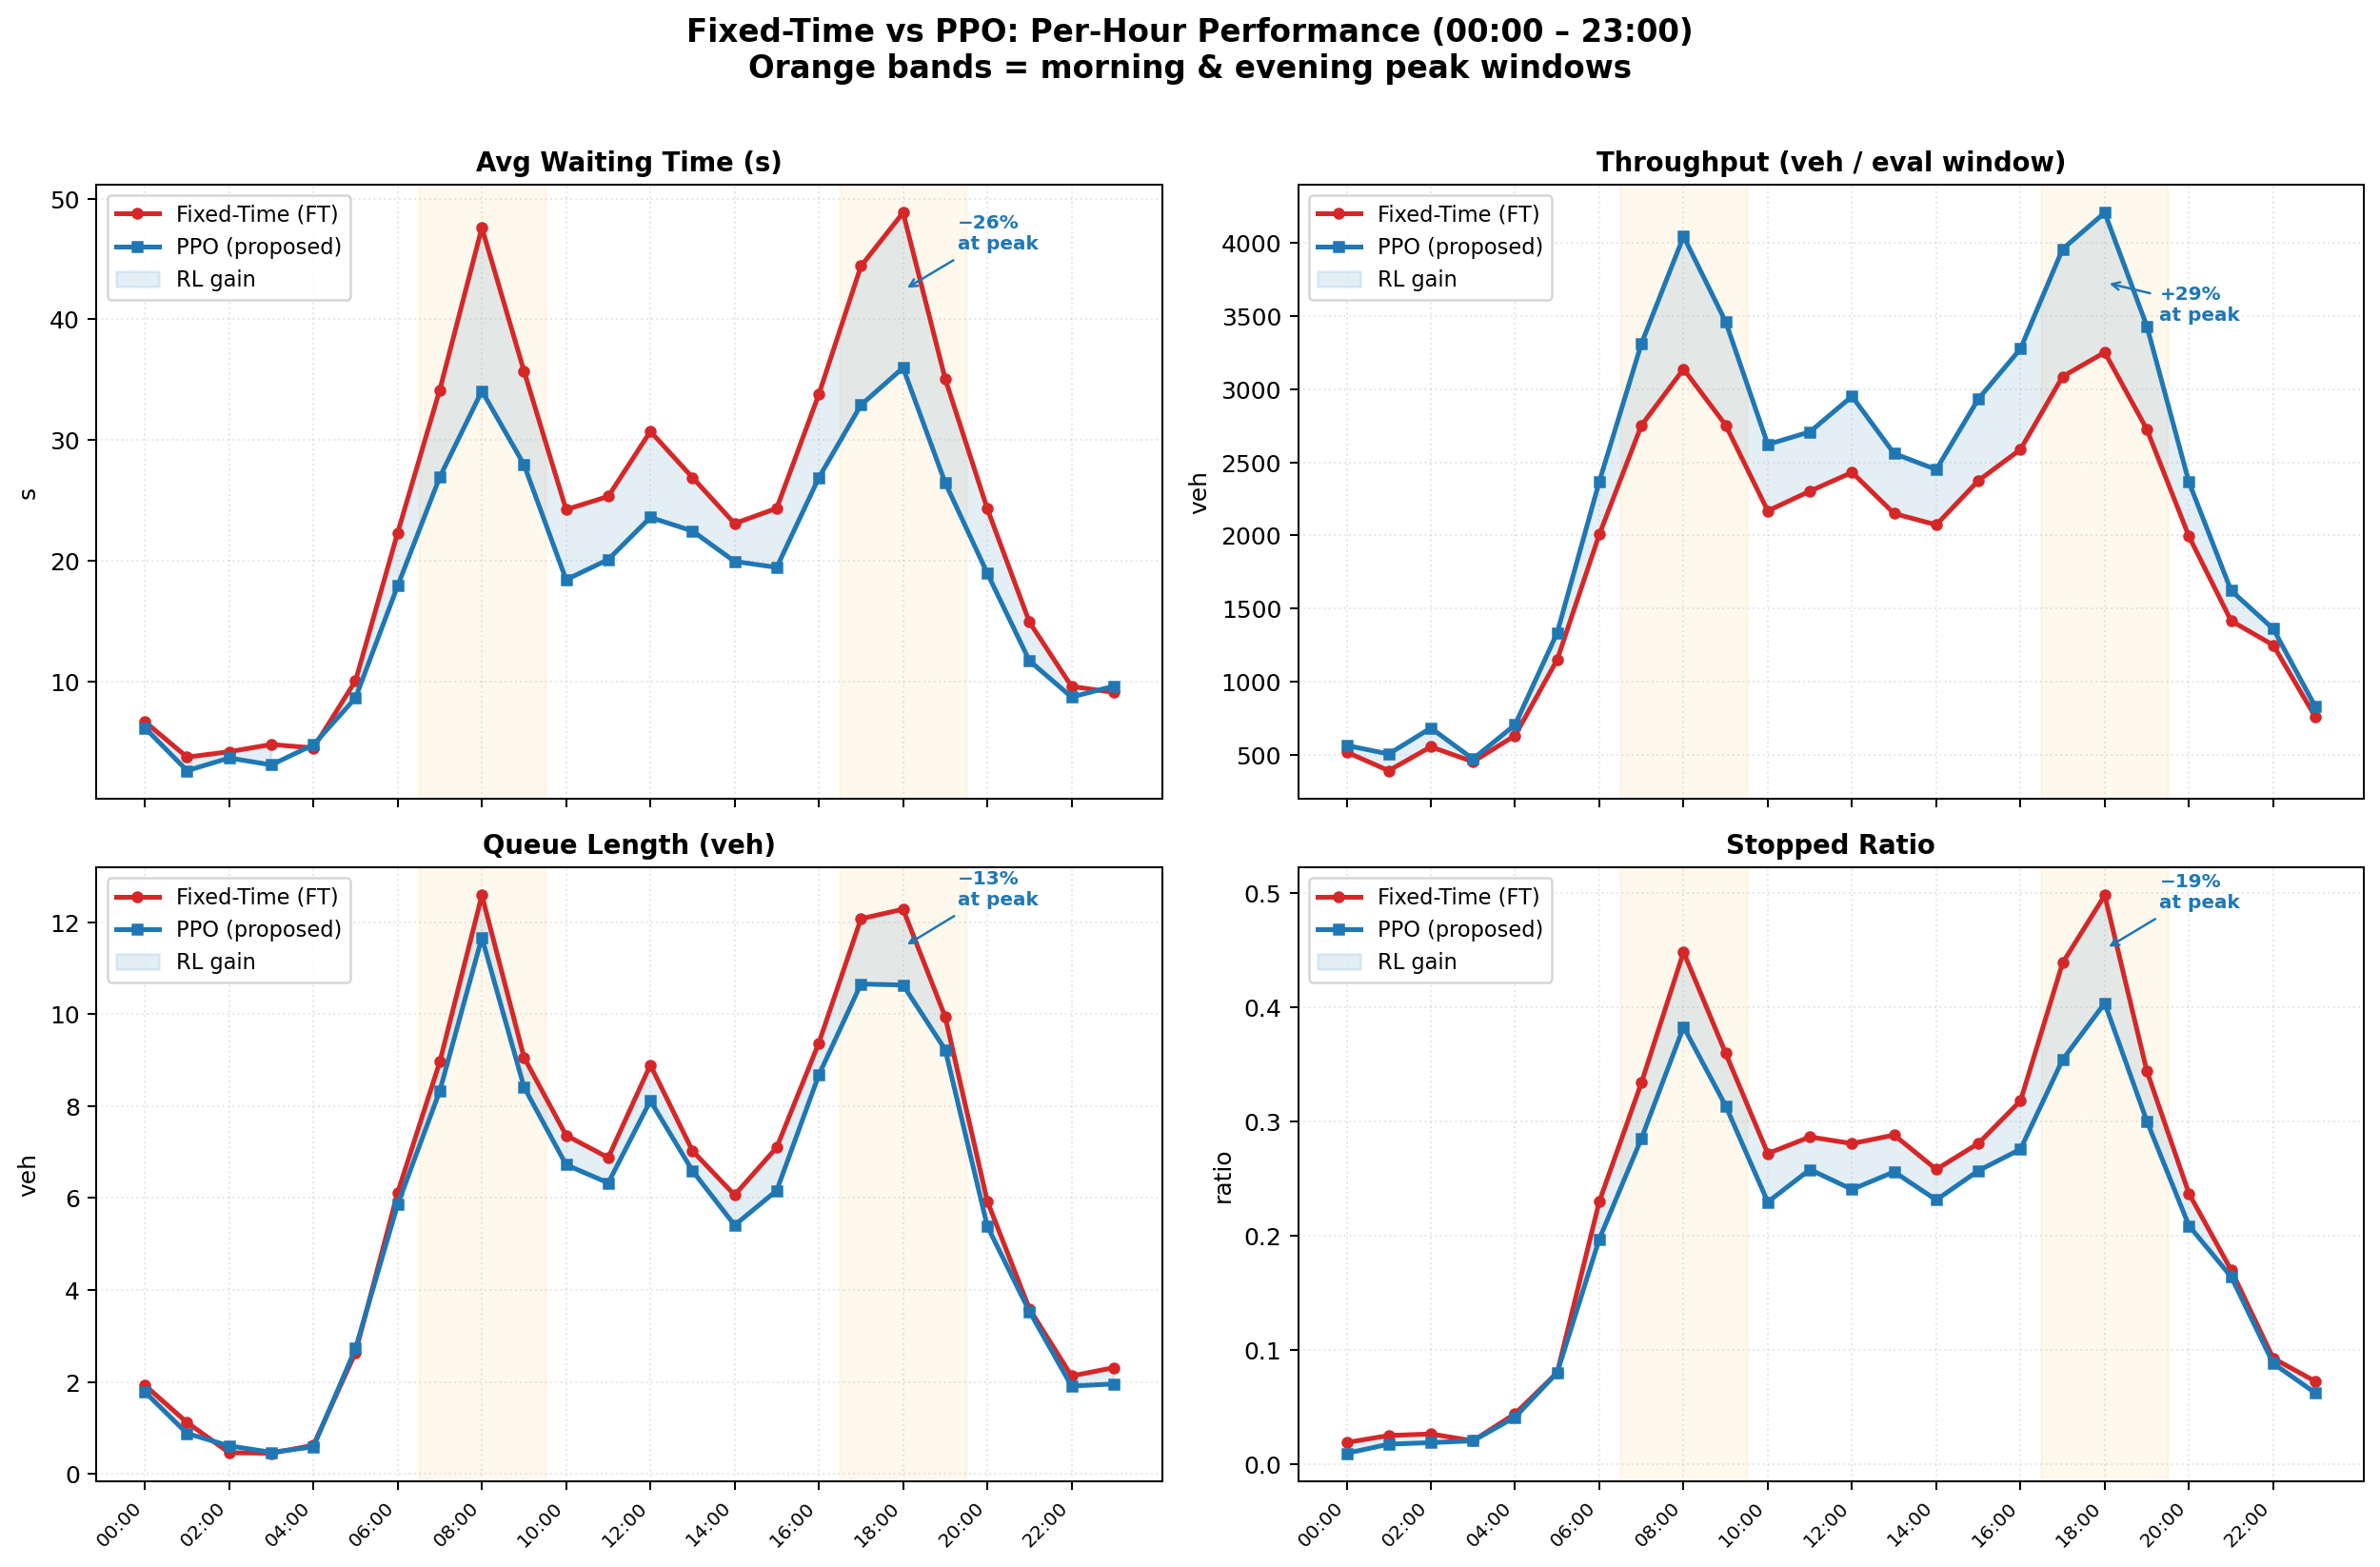
\includegraphics[width=\textwidth]{figures/fig06_hourly_comparison.png}
  \caption{Fixed-time vs.\ \ppo{} performance across all 24 hours
    (averaged over four scenarios and five seeds each).  Orange bands
    mark morning (07:00--09:00) and evening (17:00--19:00) peaks.
    The shaded region represents the \ppo{} gain; it widens
    substantially during peak hours.}
  \label{fig:hourly}
\end{figure}

\ppo{} consistently outperforms \ft{} on every metric at every
hour; however, the improvement gap widens substantially during
the morning (07:00--09:00) and evening (17:00--19:00) peak windows
(orange bands).  During these windows, vehicle arrivals exceed
the capacity of pre-programmed fixed cycles, causing
disproportionate queue build-up.  The \ppo{} agent's adaptive
phase selection exploits real-time occupancy signals to dampen
this effect.

Off-peak hours (00:00--06:00, 22:00--23:00) show smaller absolute
and relative gaps, consistent with the expectation that fixed-time
plans perform adequately under low, predictable demand.  This
result is operationally important: it suggests that the cost-benefit
case for deploying adaptive RL-based signal control is strongest at
peak hours, precisely when traffic management is most consequential.

The widening of the gain at peak hours provides further evidence
that the \ppo{} agent is genuinely adapting to demand rather than
learning a fixed timing policy that happens to perform well on
average.

\section{Ablation: Trimmed vs.\ Full Action Space}
\label{sec:res_ablation}

Preliminary experiments trained PPO with the full
\texttt{MultiDiscrete}$([6]^{12})$ action space.  The policy failed
to improve over fixed-time on \textit{main} after 300k steps,
exhibiting reward stagnation.  After trimming to
\texttt{MultiDiscrete}$([2,2,2])$ and replacing the MLP(512,512)
policy with MLP(128,128), the policy consistently converged within
200k steps.

This result confirms that action-space and network-size bloat are
significant failure modes for deep RL in traffic signal control.
Each unused action head contributes noise to the policy gradient
and inflates the variance of the actor-critic value estimate.
Trimming to the active topology eliminates this noise and reduces
the effective learning problem to a manageable size.

\section{Deployment Pathway}
\label{sec:disc_deploy}

Real-time deployment of the trained policy requires three
components:

\begin{enumerate}[leftmargin=*]
  \item A sensor backend providing halting counts and waiting
        times per lane (inductive loops, radar, or camera-based
        vehicle detection).

  \item A signal controller API equivalent to TraCI --- either a
        direct OPC-UA or NTCIP interface to the signal hardware,
        or a middleware layer that translates phase-selection
        commands to hardware.

  \item A safety conflict checker that blocks requests for
        simultaneously conflicting green phases (e.g., opposing
        left-turn movements without protected phases), ensuring
        that no learned policy can generate physically dangerous
        signal states.
\end{enumerate}

Prototype implementations of components (1) and (3) are available
in the codebase (\texttt{sensors.py} and \texttt{safety.py}).
Component (2) requires integration with the specific signal
hardware installed at each Baku intersection, which is outside the
scope of the current research but is a tractable engineering task.

\section{Comparison with Prior Benchmarks}
\label{sec:disc_compare}

Most published DRL-ATSC results are evaluated on synthetic grids
with uniform lane configurations.  The \textit{main} scenario
throughput improvement of $+31.1\%$ and \textit{Bottleneck}
waiting-time improvement of $+24.8\%$ are broadly comparable to
--- and in some metrics exceed --- reported improvements in
IntelliLight~\cite{intellilight2018}, PressLight~\cite{presslight2019},
and MPLight~\cite{mplight2020}, despite operating on topologically
irregular, real-city networks that are demonstrably harder
evaluation environments.

\section{Limitations and Validity Threats}
\label{sec:disc_limitations}

\textbf{Simulation fidelity.}
All results are obtained within SUMO.  Real-world deployment may
encounter phenomena not captured in the simulator --- sensor noise,
vehicle behaviour edge cases, and infrastructure constraints.

\textbf{Waiting-time variance.}
The high variance on waiting time across seeds of the \textit{main}
scenario (std~$\approx 22\%$) and the two congestion-collapse events
at seeds 2000 and 5000 indicate that the policy has not encountered
all relevant demand regimes during training.  Domain randomisation~\cite{domainrand2017}
over demand scale, or curriculum learning over demand intensity~\cite{curriculum2009},
could address this.

\textbf{Topology-specific policies.}
Each trained policy is specific to its scenario's TL count and phase
structure.  Transfer to a new intersection topology requires
retraining.  Transfer learning for RL~\cite{transferrl2009} and
graph neural network policies that condition on the road topology
graph are promising avenues for zero-shot transfer.

\textbf{Synthetic demand.}
Semi-synthetic demand profiles are used rather than recorded vehicle
trajectories.  The absolute demand levels are approximate; relative
comparisons between \ppo{} and \ft{} under the same seed are
unaffected.

% ============================================================
\chapter{Summary and Future Work}
\label{chap:conc}
% ============================================================

\section{Summary of Findings}
\label{sec:summary}

This thesis presented a multi-agent \ppo{} framework for adaptive
traffic signal control and evaluated it on four real-topology Baku
intersection scenarios in \sumo{}. The study was motivated by two clear
gaps in the DRL-ATSC literature: the heavy reliance on idealised grid
benchmarks and the limited use of multi-seed evaluation.

The key findings are as follows:

\begin{enumerate}[leftmargin=*]

  \item \textbf{Consistent throughput improvements.}
        \ppo{} outperforms fixed-time control on throughput across
        all four scenarios and all tested seeds, with mean
        improvements ranging from $+16.7\%$ (Pedestrian) to
        $+31.1\%$ (Main).  The 10/10 seed win rate on the primary
        \textit{main} scenario provides strong statistical evidence
        of robustness.

  \item \textbf{Composite reward is essential.}
        The ablation study confirms that naive single-metric reward
        functions (R1: queue pressure) stagnate below the fixed-time
        baseline, while the proposed 7-term composite reward (R3)
        achieves reliable convergence on all four scenarios.
        Statistical gradient analysis is a practical and principled
        method for calibrating reward weights.

  \item \textbf{Observation and action space trimming is critical.}
        Training with the full $[6]^{12}$ action space failed to
        converge in preliminary experiments; trimming to the
        active topology reduced the required training budget by
        an order of magnitude and was necessary for convergence
        on the \textit{main} scenario.

  \item \textbf{Multi-seed evaluation is indispensable.}
        Single-seed results would have been misleading in several
        instances.  Seeds 2000 and 5000 of the \textit{main} scenario
        revealed a congestion-collapse vulnerability that would be
        invisible in a single-seed evaluation on seed~42.

  \item \textbf{Metric collinearity simplifies interpretation.}
        The near-perfect Pearson correlation $r=0.9948$ between
        stopped ratio and queue length means that failures on these
        two metrics are not independent, simplifying both reward
        design and results reporting.

  \item \textbf{Peak-hour dominance of RL advantage.}
        The time-of-day analysis reveals that \ppo{} improvements
        are substantially larger during morning and evening peak
        windows, precisely when fixed-time plans are most rigid
        and congestion is most costly.

\end{enumerate}

In summary, the results show that a multi-agent \ppo{} approach can
reliably outperform fixed-time control on the four Baku scenarios used
in this thesis when it is paired with a well-calibrated composite reward
and a topology-aware action space. The gains are not limited to a single
lucky run; they remain visible across multiple demand seeds and across
several complementary traffic metrics.

\section{Contributions}
\label{sec:contributions}

This thesis makes the following original contributions:

\begin{enumerate}[leftmargin=*]
  \item \textbf{A four-scenario SUMO benchmark} with real Baku
        road topology, spanning 1--12 traffic lights and three
        traffic flow regimes --- the first such benchmark for
        Azerbaijan-based road networks.

  \item \textbf{A composite reward function} with empirically
        calibrated weights derived through per-$\sigma$ gradient
        analysis, incorporating seven terms covering all major
        aspects of intersection performance.

  \item \textbf{The \texttt{TrimmedTrafficEnv} design pattern}:
        a topology-specific observation and action space trimming
        mechanism that eliminates gradient noise and enables
        convergence with a standard MLP policy.

  \item \textbf{A ten-seed multi-seed evaluation protocol}
        for the primary benchmark scenario, establishing a
        statistical standard for honest evaluation of DRL-ATSC
        policies under stochastic demand.
\end{enumerate}

\section{Future Work}
\label{sec:future}

Several natural directions emerge from this work:

\textbf{Real traffic data integration.}
Replacing semi-synthetic demand with actual vehicle counts from
inductive loops or camera-derived flow profiles would close the
sim-to-real gap.  Challenges include vehicle re-identification
across cameras, lane-level tracking under occlusion, and data
privacy constraints.

\textbf{Transferable policies via graph neural networks.}
A GNN policy~\cite{cctv2020} built on graph convolutional~\cite{gcn2017}
or graph attention~\cite{gat2018} foundations that conditions on the
road topology graph could enable zero-shot transfer~\cite{transferrl2009}
to unseen intersection layouts, eliminating the need for per-scenario
training runs.

\textbf{Hierarchical and safe RL.}
A two-level hierarchy~\cite{hierarchicalrl2021} (network-level coordinator
+ intersection-level executor) could enable large-scale deployment.
Safety-constrained RL~\cite{saferl2015} with formal conflict shields
would ensure that learned policies never generate physically conflicting
phase assignments.

\textbf{Emergency vehicle priority.}
Priority-weighted reward terms for emergency vehicles and public
transport would address a key real-world deployment requirement
not covered in the current uniform-vehicle model.

\textbf{Pedestrian-explicit modelling.}
The \textit{pedestrian} scenario currently uses proxy slow vehicles
for pedestrians.  Using SUMO's native pedestrian model with explicit
crossing demand would make the scenario more realistic.

\textbf{Extended seed evaluation.}
Running 20--50 seeds per scenario with bootstrap confidence intervals
would provide tighter statistical estimates of population-level
performance, further strengthening the multi-seed methodology
introduced here.

\textbf{Online learning and sim-to-real transfer.}
Deploying the trained policy in a shadow mode (observing but not
controlling), collecting real-world state-action-reward tuples,
and fine-tuning the policy with a small number of online updates
could bridge the remaining gap between simulation and reality.

% ============================================================
% BIBLIOGRAPHY
% ============================================================
\clearpage
\addcontentsline{toc}{chapter}{Bibliography}

\bibliographystyle{IEEEtranDOI}
\bibliography{references}

\end{document}
